\documentclass[12pt,a4paper]{article}
\usepackage[utf8]{inputenc}
\usepackage[english]{babel}
\usepackage{amsmath}
\usepackage{amsfonts}
\usepackage{amssymb}
\usepackage{latexsym}
\usepackage{makeidx}
\usepackage{graphics}
\usepackage{lmodern}
\usepackage{hyperref}
\usepackage{subcaption}
\usepackage{pgfplots}
\usepackage{dsfont}
\usepackage{multicol}
\usepackage{xcolor}
\usepackage{booktabs}
\usepackage{float}
\usepackage{subcaption}

\pgfplotsset{width=12cm,compat=1.5}

\usepgfplotslibrary{external}

\usepackage{graphicx}
\usepackage{wrapfig}
\author{Daniel Vázquez Lago}
\usepackage{fancybox}
\title{Apuntes Óptica I}

\graphicspath{ {Imagenes/} }


\setlength{\parindent}{15px}
\usepackage[left=2.25cm,right=2cm,top=4cm,bottom=2cm]{geometry}


\newcommand{\parentesis}[1]{\left( #1  \right)}
\newcommand{\parciales}[2]{\frac{\partial #1}{\partial #2}}
\newcommand{\pparciales}[2]{\parentesis{\parciales{#1}{#2}}}
\newcommand{\ccorchetes}[1]{\left[ #1  \right]}
\newcommand{\D}{\mathrm{d}}
\newcommand{\derivadas}[2]{\frac{\D #1}{\D #2}}
\newcommand{\sech}{\mathrm{sech} \ }
\newcommand{\csch}{\mathrm{csch} \ }
\newcommand{\cotanh}{\mathrm{cotanh}}
\newcommand{\cotan}{\ \mathrm{cotan}}
\newcommand{\Res}{\mathrm{Res}}
\newcommand{\Arg}{\mathrm{arg}}
\newcommand{\Real}{\mathrm{Re}}
\newcommand{\tquad}{\quad \quad \quad}

\definecolor{color1}{cmyk}{1.0,0.0,1.0,0.05}

\newcommand{\TE}{\mathrm{TE}}
\newcommand{\TM}{\mathrm{TM}}

\newcommand{\rota}{\nabla \times}
\newcommand{\dive}{\nabla \cdot}

\newcommand{\Bn}{\mathbf{B}}
\newcommand{\En}{\mathbf{E}}
\newcommand{\Dn}{\mathbf{D}}
\newcommand{\Hn}{\mathbf{H}}
\newcommand{\Jn}{\mathbf{J}}
\newcommand{\Fn}{\mathbf{F}}
\newcommand{\fn}{\mathbf{f}}
\newcommand{\vn}{\mathbf{v}}
\newcommand{\kn}{\mathbf{k}}
\newcommand{\Kn}{\mathbf{K}}
\newcommand{\rn}{\mathbf{r}}
\newcommand{\An}{\mathbf{A}}
\newcommand{\an}{\mathbf{a}}
\newcommand{\Pn}{\mathbf{P}}
\newcommand{\pn}{\mathbf{p}}
\newcommand{\mn}{\mathbf{m}}
\newcommand{\Mn}{\mathbf{M}}
\newcommand{\Ln}{\mathbf{L}}
\newcommand{\Sn}{\mathbf{S}}
\newcommand{\Tn}{\mathbf{T}}
\newcommand{\sn}{\mathbf{s}}
\newcommand{\In}{\mathbf{I}}
\newcommand{\Gn}{\mathbf{G}}
\newcommand{\gn}{\mathbf{g}}
\newcommand{\un}{\mathbf{u}}
\newcommand{\Rn}{\mathbf{R}}
\newcommand{\hnn}{\hat{\mathbf{n}}}
\newcommand{\hnr}{\hat{\mathbf{r}}}
\newcommand{\hnz}{\hat{\mathbf{z}}}
\newcommand{\hnx}{\hat{\mathbf{x}}}
\newcommand{\hny}{\hat{\mathbf{y}}}
\newcommand{\hnu}{\hat{\mathbf{u}}}
\newcommand{\hnR}{\hat{\mathbf{R}}}


\newcommand{\bn}{\mathbf{b}}
\newcommand{\cn}{\mathbf{c}}

\newcommand{\nrho}{\boldsymbol{\rho}}


\newtheorem{theorem}{Teorema}[section]
\newtheorem{corollary}{Corolario}[theorem]
\newtheorem{lemma}{Lema}[section]
\newtheorem{ejemplo}{Ejemplo}[section]



\numberwithin{equation}{section}
\numberwithin{figure}{section}


\begin{document}

\maketitle

\newpage

\tableofcontents

\newpage

\section{Óptica Geométrica}

\subsection{Fundamentos de la óptica geométrica}

El \textbf{índice de refracción} de un medio es una propiedad intrínseca al medio de carácter adimiensional que nos da una medida de la velocidad de la luz por el mismo. Depende de la estructura de dicho medio, y existen diferentes calificaciones. En óptica:

\begin{equation}
n = \frac{v}{c}
\end{equation}

donde $v$ es la velocidad de la luz en el medio y $c$ es la velocidad de la luz en el vacío. Tiene una relación directa con la longitud de onda, ya que la velocidad de una onda electromagnética depende del medio, y como la frecuencia se conserva la longitud de onda debe cambiar. Consecuentemente podemos decir que:

\begin{equation}
n = \frac{v}{c} = \frac{\lambda}{\lambda_0}
\end{equation}

donde $\lambda_0$ es la longitud de onda en el vacío y $\lambda$ la longitud de onda en el medio. Es obvio entonces que $n(\lambda)$ depende de la longitud de onda, lo que puede ocasionar un fenómeno conocido conocido como \textbf{dispersión cromática}, que no es mas que la descomposición de la luz en sus diferentes longitudes de onda. 

\subsection{Leyes de la Óptica geométrica}

La \textbf{ley de la reflexión} nos dice que la superficie donde se produce una reflexión debe ser un plano, y que el ángulo de incidencia y el de reflexión son iguales. Podemos considerar, en una relfexión, que el índice en una reflexión es negativo $-n$. \\


La \textbf{ley de la refrección} tiene toda su base en la \textbf{ley de Snell} (de hecho son equivalentes). Esta nos dice que el ángulo con el que incide un rayo de luz y el ángulo con el que sale esta relacionado con el índice de refracción del medio de tal manera que si $\theta_1$ es el ángulo incidente y $\theta_2$ es el ángulo refractado la relación es:

\begin{equation}
n_1 \sin (\theta_1) = n_2 \sin (\theta_2)
\end{equation}

\begin{figure}[h!] \centering
\includegraphics[scale=0.08]{Refracción.pdf}
\end{figure}

Supongamos que estamos viendo un pez o un objeto sumergido en agua. Siempre va a ocurrir que el pez que nosotros podamos ver va a estar a una distancia menor de la que en realidad está (lo vemos mas cerca). Este fenómeno se puede explicar usando la ley de Snell. Supongamos que vemos el agua con un ángulo de incidencia de $\theta$ y que sale con un ángulo de incidencia $\theta'$. Lo que nosotros creemos ver es la continuación de nuestro rayo de luz. Mirando la siguiente imagen podremos deducir que obviamente la ecuación que regula la profundidad aparente $s'$ para ángulos pequeños tal que $ \tan \theta \simeq \sin \theta $  es la siguiente:

\begin{equation}
s n' = s' n
\end{equation}
donde n'=1 y n=4/3 en el caso del agua.


\begin{figure}[h!] \centering
\includegraphics[scale=0.5]{profundidadaparente.png}
\end{figure}

\newpage

\section{Óptica Paraxial}

La óptica paraxial es el estudio de la óptica para sistemas ópticos donde podemos realizar aproximaciones de primer orden, es decir, que podemos suponer la relación $\tan \theta = \sin \theta$. Es esta la aproximación que desarrollará toda la óptica posterior.\\

En un sistema óptico en general nos interesa estudiar como se comporta la luz cuando atraviesa el sistema. Si tenemos un objeto que emite rayos de luz, nos interesa saber como se comportan estos rayos de luz a la salida del objeto. \\

Es super importante tener claro lo que es un objeto y una imagen del objeto. Supongamos que tenemos un punto objeto que genera rayos de luz en varias direcciones. Llamamos al punto imagen o imagen a aquel punto donde los rayos de luz se vuelven a cruzar. Si en dicho punto pusiéramos una pantalla podríamos ver el objeto tal cual, ampliado o reducido en tamaño, pero podríamos verlo nítidamente. En el caso de poner la pantalla en otro sitio no aparecería el punto nítidamente. \\

Decimos que un objeto y una imagen son conjugados respecto al sistema óptico. Cuando decimos que dos puntos o planos son conjugados se referirán a que uno es imagen del otro a través del sistema. \\

Definimos \textbf{eje óptico} como aquella recta donde \textit{idealmente} viven el objeto y su imagen, tal que toda superficie esférica que forme parte del sistema tenga el centro de la superficie en dicha recta. En otras palabras: es la recta que une los centros de las superficies que forman el sistema óptico. Un punto lleva asociado un plano tal que se verifica que el eje óptico es la normal a dicho plano y el punto pertenece al plano. En general todo objeto que se encuentre en un plano objeto tendrá su imagen en un plano imagen. Se puede decir que son conjugados. \\

Las distancias serán positivas en el sentido que se mueve la luz y negativas en el sentido contrario al que se mueve la luz (dirección de los rayos de luz).

\subsection{Invariante de Abbe}

Cuando tenemos una superficie esférica que separa dos medios de índice de refracción diferente $n$ y $n'$, tal que la distancia del objeto a la superficie sea $s$ y la distancia de la imagen a la superficie sea $s'$, tenemos que se verifica la siguiente igualdad:

\begin{equation}
n \parentesis{\dfrac{1}{r}-\dfrac{1}{s}} = n' \parentesis{\dfrac{1}{r}-\dfrac{1}{s'}}
\end{equation}
que se llama el \textbf{invariante de Abbe}. En el caso de que la superficie esférica sea un espejo tenemos que podemos escribir que $n' = -n$ de tal modo que el invariante de Abbe de tal manera que:

\begin{equation}
\dfrac{1}{s} + \dfrac{1}{s'} = \dfrac{2}{r}
\end{equation} 

Si un objeto tiene una altura de $y$ y la imagen una altura de $y'$ podemos definir el \textbf{aumento lateral} $\beta$ como el cociente entre la altura de la imagen y la altura del objeto. Para una superficie cualquiera el aumento lateral se escribe como:

\begin{equation}
\beta = \dfrac{n s'}{n' s}
\end{equation}
además el aumento lateral total para un sistema con $k$ superficies se puede calcular como el producto de cada uno de los aumentos laterales tal que:
\begin{equation}
\beta = \beta_1 \cdot \beta_2 \cdot \ldots \cdot \beta_k
\end{equation}



\subsection{Elementos cardinales}

Existen 3 pares de puntos y 3 pares de planos asociados a estos puntos con vital importancia para el estudio de la óptica, que son \textit{puntos y planos focales}, \textit{puntos y planos principales} y \textit{puntos y planos cardinales}. Los mas relevantes para este tema serán los dos primeros. En general se estudiarán para las lentes, que son dos superficies esféricas seguidas, aunque aplica para cualquier superficie. \\

Llamamos foco objeto $F$ a aquel punto en el cual si situamos un objeto los rayos de luz al salir del sistema objeto van paralelos al eje óptico. Llamamos foco imagen $F'$ a aquel punto en el sistema imagen para el cual todas los rayos de luz de objetos situados en el infinito (es decir, rayos de luz que van paralelos al eje) coinciden. Dichos puntos \textit{no son conjugados}.  \\

Los planos principales es un par de planos conjugados (uno es imagen del otro) de tal modo que su aumento lateral es uno. Uno vive en el plano imagen y otro en el plano objeto. Es de gran utilidad, ya que si tenemos un objeto podemos trazar un rayo hacia el plano principal objeto, de tal manera que el rayo que sale después de la lente o sistema tendrá que pasar por un punto a la misma altura pero en el plano principal imagen. \\

En general toda definición de distancia se hará \textit{respecto los planos principales}. Es decir, cuando nos dicen el foco imagen está a esta distancia, nos están dando la distancia entre el plano principal imagen y el foco imagen. Lo mismo aplica para $s$, $s'$... Además asumiremos que \textit{los planos principales se encuentran confinados en el vértice}, de tal modo que podemos calcular para una superficie:

\begin{equation}
f' = r \dfrac{n'}{n'-n}; \quad f = -r \dfrac{n}{n-n'}
\end{equation}

Definimos potencia objeto $P$ y potencia imagen $P'$, que se mide en dipotrías si $f$ se mide en metros como:

\begin{equation}
P = \dfrac{n}{f} \quad P' = \dfrac{n'}{f'} \label{Ec:potencia}
\end{equation}

Los puntos cardinales y planos cardinales tienen ganancia angular uno, lo cual nos es irrelevante para esta asignatura.

\subsection{Acoplamiento de sistemas}

El acoplamiento de sistemas (sean lentes o superficies) es una herramienta básica. Supongamos que conocemos dos sistemas, con focos $F_1, F_2$, focos imagen $F_1',F_2'$, planos principales objeto $H_1,H_2$ y planos principales imagen $H_1',H_2'$. El acoplamiento de sistemas trata de reducir el problema de dos (o más) sistema a uno para el cual solo haya un sistema (por ejemplo, de dos lentes a una lente) con un solo foco objeto $F$ e imagen $F'$, y un solo par de planos principales $H$ y $H'$. \\

Definimos como \textbf{distancia de acoplamiento de planes principales} $d$ como la distancia entre los planos principales $H_1'$ y $H_2$. \\

El primer paso generalmente para calcular la ubicación de los 4 puntos tenemos que usar la \textbf{ecuación de Gullstrand} para la potencia del sistema acoplado, que será:

\begin{equation}
P = P_1 + P_2 - \dfrac{d}{n_2} P_1 P_2
\end{equation}
siendo igual para la potencia imagen. Con dicho resultado podemos calcular donde están los focos usando las ecuaciones \ref{Ec:potencia} (calculamos $f$ y $f'$). Recordando que la distancia obtenida será respecto a los planos principales del sistema equivalente, lo que debemos calcular ahora es la distancia de estos respecto a uno de los otros planos principales. Usando la ecuación:

\begin{equation}
H'H_2' = - \dfrac{d \cdot f'}{f_1'}; \quad H_1 H = \dfrac{d \cdot f}{f_2} 
\end{equation}
\subsection{Lentes delgadas}
Una lente delgada verifica que su espesor es despreciable frente a sus radios de curvatura. Dicha aproximación será una aproximación bastante útil, donde se verificarán varios puntos tales que:

\begin{itemize}
\item Los focos imagen y los focos objetos son simétricos tal que: $f = - f'$.
\item Los planos principales imagen y objeto coinciden en la propia lente.
\end{itemize}

Entonces si aplicamos el invariante de Abbe para ambas superficies tal que $d=0$ (distancia entre superficies) podemos obtener la \textbf{fórmula del constructor de lentes delgadas} que es:

\begin{equation}
\dfrac{1}{s'}-\dfrac{1}{s} =  \parentesis{\dfrac{n'-n}{n}} \parentesis{\dfrac{1}{r_1}-\dfrac{1}{r_2}} = - \dfrac{1}{f} = \dfrac{1}{f'}
\end{equation}
donde si la lente está sumergida en aire tenemos que $n=1$ y $n'$ será el índice de refracción de lo que esté hecho la lente.

\newpage

\section{Sistemas Reales}

En el estudio de sistemas reales añadiremos a la óptica paraxial (aunque posteriormente veamos un poco la óptica no paraxial) las posibles limitaciones físicas de nuestro sistema al tener un tamaño finito. Existen regiones del espacio para las cuales la luz no llega. Por ejemplo si cierras un ojo y con el otro tratas de mirar a través de una cerradura tendrás un campo de visión reducido afectado por el tamaño de la cerradura y la distancia entre tu ojo y la cerradura. \\

El estudio de la limitación de rayos es de vital importancia, y se ve afectado incluso por el tamaño finito de las lentes (es decir, las lentes pueden actuar ellas mismas como limitación del sistema). Llamamos montura al límite físico de la lente. En unas gafas podría ser el plástico que rodea a la lente. A partir de ahora a las monturas o limitaciones físicas las llamaremos \textbf{diafragmas}. \\

\subsection{Pupilas y diafragma de apertura}

Definimos como \textbf{diafragma de apertura} al orificio que limita la extensión del haz de luz que penetra en el sistema procedente de un punto objeto situado en el eje del sistema. Es un objeto real. Para calcular cual es el diagragma de apertura (D.A) tenemos que conocer cuales son las \textbf{pupilas de entrada y salida} (P.E, P.S). Definimos pupila de entrada como la imagen a través de todas las lentes anteriores (es decir, todas las lentes que van en el sentido contrario a la marcha de rayos). La pupila de salida será lo mismo pero aplicado hacia atrás. \\

Ahora bien: ¿Como calculamos la pupila de entrada y la pupila de salida? Supongamos que tenemos un objeto colocado a una distancia de nuestro sistema. La pupila de entrada será aquel objeto real o imagen que subentiende el menor ángulo con el punto del eje óptico. Para esto calculamos el cociente entre la altura de los objetos y la distancia entre punto y los objetos/imágenes. Aquel objeto que verifique el valor mínimo (que será la tangente al ángulo) será la pupila de entrada. Análogo a la pupila de salida. \\

Podemos obtener dos conclusiones de esto: la pupila de entrada depende de la distancia del objeto al sistema y que el D.A. puede ser a su vez P.E. y P.S., si es imagen de si mismo para el sistema objeto o sistema imagen. \\

\subsection{Lucarnas y diafragma de campo}

Definimos como \textbf{diafragma de campo} (D.C) al orificio que controla la extensión de campo de visión de un objeto que puede ser visto a través de un sistema óptico. Es un objeto real. Básicamente limita el tamaño del objeto que pasa por el sistema. \\

Las \textbf{lucarnas de entrada} (L.E.) y \textbf{salida} (L.S.) son las imagenes a través de parte del sistema óptico (entrada hacia el sistema objeto, salida hacia el sistema imagen) del diafragma de campo. \\

Calculamos las lucarnas como aquella imagen que subentiende el menor ángulo entre el centro de la pupila de entrada y el límite superior de la imagen. Una vez tenemos las lucarnas podemos conocer cual es el diafragma de campo. \\

Los campos de iluminación son las alturas para las cuales se empieza a limitar el tamaño del objeto. Definimos como \textbf{iluminación plena} ($O_1$) a la altura a partir la cual el objeto comienza a verse afectado por la lucarna. Definimos \textbf{iluminación límite} ($O_3$) a la altura a partir la cual la luz ya no pasa por el sistema. La \textbf{iluminación media} será el valor medio de las dos ($O_2$). La iluminación plena se calcula a partir de unir el límite superior de la L.E. con el límite superior P.E., la iluminación límite a partir de unir el límite superior de la L.E. con el límite inferior de la P.E.. La iluminación límite serla la unión del límite superior con el punto medio.

\subsection{Aberraciones}

En la óptica paraxial las imágenes son perfectas porque usamos aproximaciones de primer orden. Las aproximaciones de mayor orden dan lugar a diferencias con el comportamiento paraxial que producen aberraciones. Para las aproximaciones de tercera orden tenemos la teoría de aberraciones de Seidel. \\

A medida que abrimos los diafragmas del sistema óptico las aberraciones irán en aumento: se pierde la nitidez de los detalles, luz blanca se dispersa, los planos imagen ahora son curvos... \\

Las aberraciones de Sneidel se pueden difernciar en dos grandes grupos. Uno será las aberraciones para ondas monocromáticas y otras para las ondas crómaticas, debidas básicamente a la dependencia del índice de refracción con la longitud de onda. Las ondas monocromáticas tienen las siguientes aberraciones:

\begin{itemize}
\item Afectan a la calidad de la imagen en un punto:
\begin{itemize}
\item Aberración esférica.
\item Coma.
\item Astigmatismo.
\end{itemize}
\item Afectan a la posición de la imagen:
\begin{itemize}
\item Curvatura de campo.
\item Distorsión.
\end{itemize}
\end{itemize}

\newpage

\section{Fundamentos de la teoría electromagnética de la luz}

En este tema haremos un repaso de las leyes de Maxwell y las ecuaciones de ondas que se derivan de las mismas. Además estudiaremos el vector y teorema de Poyting, para asi definir la irradiancia y potencia de una onda, un conceptos sumamente importantes para los siguientes temas:

\subsection{Ecuaciones de Maxwell}

Como bien sabemos las ecuaciones de Maxwell son las siguientes:


\begin{subequations}\label{Ec:4.1.Maxwell}
\begin{align}
\dive \Bn & = 0 \label{Ec:4.1.a.DivB}
\end{align}
\begin{align}
\dive \En & = \dfrac{\rho}{\varepsilon_0} \label{Ec:4.1.b.DivE}
\end{align}
\begin{align}
\rota \Bn  & = \mu_0 \Jn + \mu_0 \varepsilon_0 \parciales{\En}{t} \label{Ec:4.1.c.RotB}
\end{align}
\begin{align}
\rota \En  & = -  \parciales{\Bn}{t} \label{Ec:4.1.d.RotE}
\end{align}
\end{subequations}
donde $\rho \equiv$ densidad de carga $[C/m^3]$ y $\Jn \equiv$ densidad de corriente de carga $[C/m^2 s]$. El campo eléctrico es $\En$ medido en $[V/m+$ y el campo magnético es $\Bn$ medido en $[T] \equiv [V s/ m^2]$. De estas ecuaciones se deducen a su vez las ecuaciones de ondas, una para el campo eléctrico y otra para el campo magnético. Suponemos que el lector conocerá de sobra la deducción de estas.


\subsection{Ecuación de ondas}

La ecuación de ondas espacial espaciales si los campos están suficientemente lejos de las fuentes ($\Jn,\rho \rightarrow 0$) son las siguientes:


\begin{subequations}
\begin{equation}
\nabla^2 \En - \mu_0 \varepsilon_0 \parciales{\En}{t^2} = 0 \label{Ec:4.2.a.Ondas}
\end{equation}
\begin{equation}
\nabla^2 \Bn - \mu_0 \varepsilon_0 \parciales{\Bn}{t^2} = 0 \label{Ec:4.2.b.Ondas}
\end{equation}
\end{subequations}  


En general el estudio de las ondas lleva al estudio de dos casos: el caso en el que los campos solo se propagan por una dirección dada (onda plana) y que solo se propague por la coordenada radial. \\

Supongamos que una onda se propaga con dirección $\sn$. Esto es equivalente a decir que solo depende de la coordenada $\zeta$ que gobierna dicha dirección. Ahora bien, por las propiedades del producto escalar podemos calcular la $\zeta$ de cada punto del espacio como $\zeta = \sn \cdot \rn$. Entonces tendríamos que $\En (\rn,t) = \En ( \rn \cdot \sn, t) = \En (\zeta, t)$. \\

Podemos suponer sin pérdida de generalidad que la dirección $\sn$ es paralela al eje $\hnx$.  En ese caso la ecuación de ondas se convierte en una ecuación de ondas escalar tal que:

\begin{equation}
f_{xx} - \dfrac{1}{c^2} f_{tt} = 0 \Longrightarrow f(x,t) = f_+ (x-ct) + f_- (x+ct)
\end{equation}

Queda claro entonces que $c= 1/\sqrt{\varepsilon
_0 \mu_0}$ para las ondas electromagnéticas. A continuación reescribimos las ecuaciones en las coordenadas mas generales, tal que la solución queda en:

\begin{equation}
f(\sn \cdot \rn,t) = f_+ (\sn \cdot \rn-ct) + f_- (\sn \cdot \rn +ct)
\end{equation}
siendo este tipo de ondas las \textbf{ondas planas}. Las ondas esféricas donde el campo dependería de $\En (\rn,t) = \En (r,t)$ son un poco mas complicadas ya que la ecuación de ondas es la siguiente:

\begin{equation}
\dfrac{1}{r} (rf)_{rr} - \frac{1}{c^2} f_{tt} = 0  
\end{equation}
de lo que se deduce que la solución mas general de la ecuación de ondas es:

\begin{equation}
f(r,t) = \dfrac{f_+ (r-ct)}{r} + \dfrac{f_- (r+ct)}{r}
\end{equation}

Como podemos ver este tipo de ondas divergen cuando $r$ tiende a cero. Debemos pensar que las ecuaciones de ondas que hemos presentado son las ecuaciones de ondas para campos lejos de las fuentes, por lo que si realmente estudiamos el campo cerca de la emisión de estas las ecuaciones usadas no serán ni por asomo válidas. \\

\subsection{Ondas monocromáticas}

La solución mas sencilla para las ecuaciones de ondas son las \textit{ondas armónicas} que vienen dadas por funciones sinusoidales tal que:

\begin{equation}
f(\rn,t) =  A(\rn) cos ( \phi(\rn) - \omega t) 
\end{equation}
donde $\omega$ es la frecuencia angular onda. La frecuencia angular esta relacionada con el inverso del periodo $T$ tal que $T = 2 \pi / \omega$, siendo el periodo el tiempo que para un punto fijo la perturbación vuelve a ser igual, i.e. mide el tiempo que trascurre entre máximo y máximo para un mismo punto. \\

Al término que va dentro del coseno lo llamamos \textbf{fase} ($\Phi = \phi(\rn) - \omega t)$) y al término que está multiplicando el coseno lo llamamos \textbf{amplitud} ($A(\rn)$). \\

Recordemos que $A(\rn)$ es una función que depende del problema. Para las ondas planas será una constante y para las ondas esféricas proporcional a $1/r$. A continuación estudiamos las soluciones armónicos para los dos casos mas generales que hemos visto.  \\

Definimos onda monocromática como aquella solución para la cual $\omega$ es única. Por ejemplo si tenemos que solucionar el comportamiento del campo eléctrico con varias frecuencias/número de ondas tendremos que la onda ya no será una onda monocromática.

\subsubsection{Ondas armónicas planas}

Para una onda plana la solución armónica mas general, con una propagación en la dirección $\sn$, y una dirección de perturbación $\hnn$ tal que $\sn \perp \hnn$ vendrá dada por:

\begin{equation}
\En = E_s \hnn \tquad E_s(\sn\cdot\rn,t) = E_0 \cos ( \kn \cdot \rn - \omega t + \varphi) \sn  \tquad \kn = \frac{\omega}{c} \sn \quad |\kn| = k = \omega / c
\end{equation}

A este término $k$ lo llamaremos \textbf{número de onda}, y su inverso $\lambda = 2 \pi / k$ representa la distancia para un tiempo fijo entre máximo y máximo (o mínimo y mínimo) a lo largo de la dirección $\sn$. Al vector $\kn$ lo llamamos \textbf{vector número de onda} y nos da una medida del número de onda y la dirección de propagación de la onda plana.  \\


 El valor $\varphi$ es el valor del desfase que depende de las condiciones iniciales, al igual que el valor $E_0$ depende de las condiciones iniciales (son datos del problema). El primero cobra vital importancia cuando una onda pasa de un medio a otro.  \\
 
 
Una onda no puede vibrar en la dirección de propagación. Esto es un resultado implícito en las ecuaciones de Maxwell, y válido para \textit{cualquier tipo de onda}, ya que la divergencia en ese caso sería no nula (para fuentes alejadas debe cumplirse). Los campos eléctrico y magnético no pueden ser paralelos ya que uno es el rotacional del otro. Lo que si es único de las ondas planas es la relación intrínseca entre $\Bn$ y $\En$, causada por los rotacionales de las ecuaciones de Maxwell, que nos dice que:

\begin{equation}
\Bn = \dfrac{1}{\omega} \kn \times \En ; \tquad B = \dfrac{1}{v_p} E
\end{equation}
sea cual sea la velocidad de propagación del medio ($c$ si es el vacío, otro valor para otros medios). 


\subsubsection{Ondas armónicas esféricas}


Las ondas esféricas tienen la siguiente forma:

\begin{equation}
\En (r,t) = E(r,t) \hnn \tquad E(r,t) = \dfrac{E_0}{r} \cos (kr-\omega t + \delta) \tquad k = \omega/c
\end{equation}
donde $\hnn$ es perpendicular al vector de propagación $\hnr$.

 

\subsubsection{Mas allá de las ondas planas}

No obstante uno puede pensar que el interés de las ondas harmónicas es muy reducido: ¿Que pasa si la perturbación es una gaussiana o una onda cuadrada? Uno podría decir que nada de ni de la frecuencia, ni del número de onda tendría sentido, que tendríamos que solucionar la nueva ecuación de cero creando nuevas definiciones etc... \\

Nada mas lejos de la realidad, ya que gracias al genio matemático Fourier sabemos que podemos expresar cualquier \textit{función periódica} como una suma de funciones sinusoidales discretas (series de Fourier) tal que sería la suma de senos (o cosenos) con frecuencias $\omega_0,\omega_1...$ donde cada uno se llamaría \textbf{armónico}, y serían múltiplos del armónico fundamental $\omega_0$. \\

Incluso podríamos expresar una perturbación no periódica como una perturbación gaussiana mediante la trasformada de fourier que nos llevaría a la sorprendente conclusión de que en realidad dicha perturbación no es otra cosa que la suma de ondas planas pero ahora en un rango continuo en la frecuencia. \\

Es entonces de vital importancia no solo entender el aparato de Fourier si no comprender que es una onda plana o una onda monocromática, como funciona con el número de onda y la frecuencia.

\subsubsection{Representación compleja}

La representación compleja de las ondas hace sumamente cómodo estudiar las ondas armónicas, ya que hacen que estudiar el desfase muy sencillo, y por tanto lo hace vital en el estudio de la superposición de ondas y en el estudio de las superficies de separación. \\

La representación compleja sin embargo tiene un problema intrínseco asociado: en la realidad no medimos números complejos, solo números reales. Por tanto cuando representamos una onda con números complejos debemos entender que realmente lo que estamos haciendo es una caracterización puramente matemática que facilita el estudio de la realidad. \\

De hecho el campo medido normalmente se asocia con la parte real de un campo complejo, tal que:

\begin{equation}
\En (\rn,t) = \Real [\En_C (\rn,t) ]
\end{equation}
Se hace natural entonces representar nuestro campo como:

\begin{equation}
\En (\rn,t) = \An (\rn,t) \cos (\phi(\rn,t)) = \dfrac{1}{2} \parentesis{\An e^{i \phi} + \An e^{- i \phi}}
\end{equation}
Para una onda plana:

\begin{equation}
\En_C (\rn,t) =  \An \parentesis{e^{i ( \kn \cdot \rn - \omega t + \delta)}}
\end{equation}

\subsection{Energía de las ondas}

La energía que trasportan las ondas electromagnéticas es sumamente importante. Es muy importante por dos razones: saber si a través de cierto medio se pierde energía y cuanta o como se pierde es fundamental a la hora de decidir si queremos usar un material u otro. Además como la energía sabemos que es una cantidad que se conserva en la naturaleza su estudio puede llegar a solucionar algún problema. \\

Definimos el \textbf{vector de Poyting} $\Sn$ como el \textit{vector flujo de energía}, es decir, la cantidad de energía por unidad de superficie y tiempo que trasporta una onda electromagnética. Se relaciona con los campos electromagnéticos de la siguiente forma:

\begin{equation}
\Sn =  \dfrac{1}{\mu_0} \En \times \Bn = S \sn
\end{equation}
tal que $\sn$ es el vector de propagación de la onda. El \textbf{teorema de Poyting} realciona el flujo de energía que llega a un sistema a través de los campos con la energía de dicho sistema (energía mecánica o energía almacenada en los campos). Este teorema dice que:

\begin{equation}
\dfrac{\D}{\D t} (W+K) = - \int_A \S \D \an
\end{equation}
donde $K \equiv$ energía almacenada en los campos y $W \equiv $ energía mecánica. Definimos a partir del vector de Poyting las siguientes cantidades: \textbf{irrandiancia} $I$ que es el promedio temporal del flujo de energía y la \textbf{potencia} $P$ que es la cantidad de irradiancia que atraviesa una supeficie:

\begin{equation}
I = \langle S \rangle = \dfrac{1}{T_D} \int_t^{t+T_D} S \D t \quad T_D \gg T \tquad P = \int_A I \sn \cdot \D \an 
\end{equation}





\newpage

\section{Propagación de la luz en la materia}

En este tema vamos a estudiar como se comporta la luz en dos de los medios mas importantes: los dieléctricos y los conductores. El estudio de estos requerirá un análisis profundo del comportamiento del número de onda, de la frecuencia y de la amplitud. Para esto introduciremos primero las ecuaciones de Maxwell en presencia de medios con efectos como la magnetización (imanes) y la polarización. Además introduciremos los conceptos de velocidad de grupo y velocidad de fase tan importantes en la física. 

\subsection{Ecuaciones de Maxwell en la materia}

Las ecuaciones de Maxwell en la materia implica introducir dos conceptos fundamentales: la polarización y la magnetización (que aún que a la mayoría os debería sonar vamos a darle un pequeño repasillo). \\

\subsubsection{Polarización}

La \textbf{polarización} es un fenómeno en el cual los momentos dipolares de los átomos de un medio se alinean produciendo un campo eléctrico observable. Dicho fenómeno, bastante complejo, se suele describir creando las llamadas ``cargas ligadas'', teniendo así cargas libres (cargas como las que hemos visto hasta ahora) y cargas ligadas (superficiales y volumínicas). Sin entrar en detalle, si definimos la polarización volumínica como $\pn$ (momento dipolar por unidad de volumen) tal que la polarización de una región del espacio es $\Pn = \int \pn \D V$ dichas cargas se calculan como:

\begin{equation}
\rho_{b} \equiv - \dive \Pn \tquad \sigma_b \equiv \hnn \cdot \Pn
\end{equation}
donde el subíndice $b$ viene del inglés \textit{bound} (atado). Resulta entonces natural la definición de un campo eléctrico únicamente generado para las cargas libres $\Dn$ y otro para la suma de ambas cargas, que será el campo eléctrico $\En$, tal que:

\begin{equation}
\Dn = \varepsilon_0 \En + \Pn \tquad \dive \Dn = \rho_f \quad \dive \En = \dfrac{\rho_f + \rho_b}{\varepsilon_0}
\end{equation}
ya que $\rho_f$ son las cargas libres (subíndice $f$ del inglés \textit{free} que significa \textit{libre}). Cunado un medio es \textbf{lineal, homogéneo e isótropo} (medio l.h.i.) tendremos que la relación entre $\Dn$ y $\En$ será una relación lineal dada por una constante $\varepsilon$ que será la \textbf{permetividad eléctrica del medio} tal que:

\begin{equation}
\Dn = \varepsilon \En \tquad \varepsilon = (1+\chi_E) \varepsilon_0
\end{equation}

\subsubsection{Magnetización}

La magentización es algo parecido a la polarización, pero para el campo magnético. Cuando el momento dipolar de los átomos se alinean en presencia de un campo magnético externo (fenómeno que se produce para maximizar la energía del campo magnético) se produce un campo magnético perceptible, que aumenta o reduce el campo magnético externo. Nunca se produce magnetización sin un campo magnético externo, aunque muchas veces las dicho campo magnético aparece un remanente, produciendo materiales con un campo magnético intrínseco llamados imanes. \\

Para estudiar la magnetización creamos lo que llamamos ``corrientes ligadas'', teniendo corrientes libres ($\Jn_f, \Kn_f$) y corrientes ligadas ($\Jn_b,\Kn_b$). Si la magnetización por unidad de volumen  (cantidad de momento magnético por unidad de volumen) es $\mn$ tenemos que la magnetización $\Mn = \int \mn \D V$ tal que las corrientes se definen como:

\begin{equation}
\Jn_b \equiv \rota \Mn \tquad \Kn_b \equiv \Mn \times \hnn
\end{equation}

Al igual que antes resulta natural definir un campo magnético definido únicamente por las corrientes libes ($\Hn$) y otro para ambas corrientes, tal que:

\begin{equation}
\Hn = \Bn/\mu_0 - \Mn \tquad
\end{equation}

Cuando un medio es \textbf{lineal, homogéneo e isótropo} (medio l.h.i.) tendremos que la relación entre $\Hn$ y $\Bn$ será una relación lineal dada por una constante $\mu$ que será la \textbf{permeabilidad magnética del medio} tal que:

\begin{equation}
\Hn = \Bn / \mu \tquad \mu = (1+\chi_B) \mu_0
\end{equation}


\subsubsection{Ecuaciones de Maxwell en medios materiales}

En este contesto queda claro que las ecuaciones de Maxwell se reducen a:



\begin{subequations}\label{Ec:5.1.Maxwell}
\begin{align}
\dive \Bn & = 0 \label{Ec:5.1.a.DivB}
\end{align}
\begin{align}
\dive \Dn = \rho_f \label{Ec:5.1.b.DivD}
\end{align}
\begin{align}
\rota \Hn  & =  \Jn_f + \parciales{\Dn}{t} \label{Ec:5.1.c.RotH}
\end{align}
\begin{align}
\rota \En  & = -  \parciales{\Bn}{t} \label{Ec:5.1.d.RotE}
\end{align}
\end{subequations}

O también a las siguientes ecuaciones, completamente análogas:



\begin{subequations}\label{Ec:5.1.8.Maxwell}
\begin{align}
\dive \Bn & = 0 \label{Ec:5.1.8.a.DivB}
\end{align}
\begin{align}
 \varepsilon_0 \dive \En + \dive \Pn = \rho_f \label{Ec:5.1.8.b.DivE}
\end{align}
\begin{align}
\rota \parentesis{\dfrac{\Bn}{\mu_0}-\Mn}  & =  \Jn_f + \varepsilon_0 \parciales{\En}{t} + \parciales{\Pn}{t} \label{Ec:5.1.8.c.RotB} 
\end{align}
\begin{align}
\rota \En  & = -  \parciales{\Bn}{t} \label{Ec:5.1.8.d.RotE}
\end{align}
\end{subequations}

\subsubsection{Condiciones de frontera} \label{Subsub:5.1.4}

Las condiciones de frontera son fundamentales a la hora de estudiar el comportamiento de las ondas al pasar de un medio a otro, ya que la presencia de corrientes superficiales o cargas superficiales altera profundamente dichas ecuaciones. Sea una superficie de separación que separa dos regiones del espacia que llamamos región $2$ y región $1$, tal que el vector normal a la superficie apunta hacia 2. En ese caso las condiciones para los campos $\En$ y $\Bn$ son las siguientes:


\begin{equation}
\hnn \cdot (\Dn_2 - \Dn_1) = \sigma_f \tquad \En_{t2}-\En_{t1}=0
\end{equation}

\begin{equation}
\hnn \cdot (\Bn_2-\Bn_1)=0  \tquad \hnn \times (\Hn_2 - \Hn_1) = \Kn_f; \quad \Hn_{t2} - \Hn_{t1} = \Kn_f 
\end{equation}

Dado que de ahí se pueden deducir las ecuaciones para los campos $\En,\Bn$ escribimos las condiciones de frontera para dos medios l.h.i. diferentes:


\begin{equation}
\hnn \cdot (\varepsilon_2 \En_2 - \varepsilon_1 \En_1) = \sigma_f \tquad \En_{t2}-\En_{t1}=0
\end{equation}

\begin{equation}
\hnn \cdot (\Bn_2-\Bn_1)=0  \tquad \hnn \times (\Bn_2 / \mu_2 - \Bn_1 / \mu_1) = \Kn_f; \quad \Bn_{t2} / \mu_2 - \Bn_{t1} / \mu_1 = \Kn_f 
\end{equation}



\subsubsection{Energía para medios materiales}

Las ondas planas en medios l.h.i. permiten ampliar la definición del vector de Poynting y la irradiancia. Primero definiremos la \textbf{impedancia característica} del medio, que es básicamente:

\begin{equation}
Z = \sqrt{\dfrac{\varepsilon}{\mu}} = \varepsilon_0 c \sqrt{\frac{\varepsilon_r}{\mu_r}}= \varepsilon_0 c n
\end{equation}
donde $Z_0$ es la impedancia característica del vacío. En ese caso tendríamos que $n=1$. El número $Z$ puede ser complejo. Dado la relación intrínseca entre los campos electromagnéticas podemos escribir el vector de propagación como:

\begin{equation}
\Sn = \dfrac{1}{\mu} \dfrac{1}{\omega} \En \times ( \kn \times  \En ) = \dfrac{k}{ \mu \omega} | \En |^2 \sn  = Z |\En| ^2 \sn
\end{equation}

Si consideramos ondas monocromáticas tenemos que el promedio temporal de la onda verifica que el promedio temporal de l

a onda electromagnética viene dada por:

\begin{equation}
I = \langle S \rangle = \varepsilon c^2 \langle | \En \times \Bn | \rangle = \dfrac{1}{2 \mu} \Real ( \En \times \Bn^*)| = \dfrac{1}{2}  Z |\En|^2 = \dfrac{1}{2} \dfrac{1}{Z} |\Bn|^2 \label{Ec:5.1.5.013-Irradiancia}
\end{equation}

\subsection{Medios dieléctricos}

Los medios dieléctricos son aquellos medios que presentan polarizaciones macroscópicamente visibles, pero ni son conductores (aislantes eléctricos), ni presentan cargas libres. Además no son medios magnéticos (magnetización nula). \\

Como ya hemos definido si un medio es lineal (relación lineal $\Pn \propto \En$), homogéneo (propiedades iguales en todo punto del espacio) e isótropo (polarización paralela  $\Pn \parallel \En$), la relación entre polarización y campo eléctrico es una relación lineal exactamente igual en todo punto de dicho medio material, tal que:

\begin{equation}
\Pn =  \varepsilon_0 \chi \En
\end{equation}

Sin embargo dicha relación lineal depende intrínsecamente de la frecuencia (excepto para el vacío). Ello no implica que deje de ser lineal, isótropo o homogéneo; solamente dice que para cada onda la relación \textit{es diferente}. Es decir nuestra ecuación realmente viene dada por:

\begin{equation}
\Pn (\omega) = \varepsilon_0 \chi (\omega) \En (\omega)
\end{equation}
donde $\chi$ es la \textbf{susceptibilidad eléctrica}. Por simplicidad no escribimos la dependencia con $\rn$. Para hallar la relación temporal tendremos que usar la \textit{transforamda de Fourier} tal que:

\begin{equation}
\Pn (t) = \varepsilon_0 \int_{-\infty}^\infty \chi (\omega) \En (\omega) e^{-i \omega t} \D \omega
\end{equation}

Si $\bar{\chi} (t)$ es la trasformada de Fourier de $\chi (\omega)$, tendremos que la \textit{convolución de Fourier} nos permite escribir la relación anterior como:

\begin{equation}
\Pn (t) = \varepsilon_0 \int_{-\infty}^{\infty} \bar{\chi} (t-t') \En (t') \D t'
\end{equation}

Esta expresión indica que la polarización inducida está \textit{retardada} respecto el campo eléctrico, o lo que es lo mismo: la respuesta del medio a la perturbación electromagnética no es instantánea, lo que cabe esperar. Esta relación temporal no local se debe a la característica dispersiva de los medios, que hace que los medios a frecuencias suficientemente altas aparezcan respuestas retardadas. Consideraremos este fenómeno nulo. Esto equivale a considerar $\bar{\chi(t)}$ por una constante multiplicado por una constante, de tal modo que:


\begin{equation}
\Pn (t) =  \varepsilon_0 \chi \En (t)
\end{equation}

\subsubsection{Ondas planas y monocromáticas}

Como en los medios dieléctricos l.h.i $\Mn$ es cero y $\Pn = \varepsilon_0 \chi \En$, tenemos que la ecuación de ondas acaba resultando en:


\begin{equation}
\nabla^2 \En - \varepsilon_0 \mu_0 \En_{tt} - \mu_0 \Pn_{tt} = 0 \longrightarrow  \nabla^2 \En - \varepsilon_0 \mu_0 (1+\chi) \En_{tt} = 0
\end{equation}

Si definimos la permeabilidad dieléctrica del medio $\varepsilon$ como $\varepsilon  \equiv (1+\chi) \varepsilon_0$  tal que la velocidad de propagación de la onda electromagnética sea $v_p = 1/\sqrt{\mu_o \varepsilon}$, podemos reescribir la ecuación tal que:

\begin{equation}
\nabla^2 \En - \dfrac{1}{v^2_p} \En_{tt} = 0
\end{equation}

Muchas veces se define la \textbf{permeabilidad dieléctrica relativa} $\varepsilon_r$ tal que $\varepsilon_r \equiv (1+\chi)$ así $\varepsilon \equiv \varepsilon_r \varepsilon_0$. Es entonces evidente que para una onda plana cualquiera tal que $$\En = \An e^{-i (\kn \cdot \rn - \omega t)} \quad \kn = k \sn$$
debe verificarse que 

\begin{equation}
k = \dfrac{\omega}{v_p} = \dfrac{\omega}{c} n \tquad n = \dfrac{c}{v_p}
\end{equation}
siendo $n$ es lo que llamamos \textbf{índice de refracción del medio}, y se relaciona con la permeabilidad relativa tal que 

\begin{equation}
n = \sqrt{\varepsilon_r}
\end{equation}

\subsubsection{Absorción de la radiación}

Uno de los efectos mas notables resultantes de la propagación de la radiación electromagnética en la materia es la absorción de la misma. Este proceso conlleva a la disminución gradual de la energía, que se trasforma en movimiento de cargas (efecto Joule) o en la aparición de corrientes.  \\

La \textit{Ley de Bouguer} o \textit{Ley de Lambert-Beer} es una ley que es capaz de describir muy satisfactoriamente cualquier fenómeno de absorción usando la absorción de la energía (irradiancia) de un medio para cuantificar la absorción. Dicha ecuación es una ecuación exponencial que viene determinada por la siguiente ecuación diferencial lineal de primer orden:

\begin{equation}
\D I = - \alpha I \D z
\end{equation}
donde $\alpha$ es el \textbf{coeficiente de absorción}. Esta ecuación puede integrarse llegando a que la irradiancia en un medio viene dada por:

\begin{equation}
I(z) = I_0 e^{- \alpha z} \tquad I_0 \equiv I (0)
\end{equation}
Ahora podemos entender mejor el interés de definir la irradiancia y el vector de Poyting: nos permite describir la atenuación  de la luz en función de la profundidad en un medio absorbente. Al inverso del coeficiente de absorción se le llama \textbf{profundidad de penetración} 

\begin{equation}
\delta = \dfrac{1}{\alpha}
\end{equation}
que denota la distancia 

\subsubsection{Índice de refracción complejo y absorción}

Hemos considerado las relaciones entre polarización eléctrica y campo eléctrico tomando la relación para frecuencias bajas y la hemos generalizado para todo el espectro de frecuencia. Ahora vamos a reconstruir la relación para la los medios abosrbentes. \\

Como hemos mencionado anteriormente a altas frecuencias el medio no es capaz de responder instantáneamente a estas variaciones del campo. Eso lleva a que exista una relación de desfase si la onda es monocromática, tal que para la notación real:

\begin{equation} 
\left.
\begin{array}{l}
\En (t) = \En_0 \cos (\varphi_e - \omega t) \\
\Pn (t) = \Pn_0 \cos (\varphi_p - \omega t) 
\end{array} \right\rbrace \Longrightarrow \Pn (t) = \Pn_0 \cos (\varphi_e + \Delta \varphi - \omega ) \tquad \Delta \varphi = \varphi_p - \varphi_e
\end{equation}
donde claramente $\Delta \phi$ es el retraso, el desfase entre polarización y campo eléctrico. Se supone que como las amplitudes son proporcionales, tenemos que, escribiendo en números complejos, la relación:

\begin{equation}
\Pn (t) =  \varepsilon_0 \gamma (\omega) e^{i \Delta \varphi} \En_0 e^{i (\varphi_e - \omega t)}
\end{equation}

Como podemos ver esto implica necesariamente que la \textit{susceptibilidad eléctrica} sea un número complejo, tal que:

\begin{equation}
\chi (\omega) = \gamma (\omega) e^{i \Delta \varphi}
\end{equation}

Una susceptibilidad eléctrica compleja implica una permitidividad relativa compleja, por lo que habrá un índice de refracción complejo, y que:

\begin{equation}
n_C = \sqrt{1+\chi} = n + i \kappa
\end{equation}
donde $\kappa$ es la parte imaginaria que se relaciona con el coeficiente de absorción, y $n$ es el índice de refracción normal mediando la velocidad de propagación respecto la velocidad de la luz. En ese caso tendremos que:

\begin{equation}
\En = \An e^{i \kn \cdot \rn - \omega t} = \An e^{-\kappa \frac{\omega}{c} \sn \cdot \rn} e^{i \parentesis{n \frac{\omega}{c} \sn \cdot \rn - \omega t}}
\end{equation}

Como sabemos la irradiancia en ondas planas queda definida por la ecuación \ref{Ec:5.1.5.013-Irradiancia}, tal que en ese caso:

\begin{equation}
I = \dfrac{|n_C|}{2 \mu_0 c} |\En|^2  = \dfrac{|Z|}{2} E_0^2 e^{-2 \frac{\omega}{c} \kappa ( \sn \cdot \rn)}
\end{equation}
de tal modo que podamos relacionar $\alpha$ con $\kappa$ tal que:

\begin{equation}
\alpha = 2 \dfrac{\omega}{c} \kappa = \dfrac{4 \pi}{\lambda
} \kappa
\end{equation}

\subsubsection{Ondas no monocromáticas y velocidad de grupo}

Tal y como hemos visto ahora las ondas monocromáticas son ondas perfectas, ideales, sin principio ni fin: no existe como tal un frente de ondas, la onda se encuentra en todas partes instantáneamente. Una onda real es generada en un determinado momento y se desvanece cuando es atenuada por su interacción con la materia.  \\

Solo para una onda real tiene sentido preguntarse cuanto tarda en propagarse, o lo que es lo mismo, cual es la velocidad. Resulta que la velocidad de fase $v_p = \omega / k(\omega)$ no es la respuesta, ya que esta indica como se mueven las superficies de fase constante. En este apartado vamos a ver que la velocidad de propagación esta asociada a la dispersión de un medio depende del índice de refracción y su relación con la frecuencia. \\

Como sabemos la relación intrínseca entre el campo eléctrico en función del tiempo y en función de  la frecuencia se relaciona únicamente por la integral de Fourier tal que:

\begin{equation}
E(z,t) = \int_{-\infty}^{\infty} A(\omega) e^{i(k(\omega)z - \omega t + \varphi (\omega))} \D \omega
\end{equation}
donde separamos el número de onda en $k(\omega) = n(\omega) \omega c$. Sea la onda un paquete de ondas centrado en $\omega_0$, con un número de onda $k_0$ para dicha frecuencia $k_0 \equiv k(\omega_0)$, y una anchura de $\Delta \omega$. Si realizáramos la integral en un instante determinado $t_0$ obtendríamos un paquete localizado en torno a un punto $z=z_0$. En un instante posterior dicho paquete estará localizado en otro punto del eje $z$. La velocidad del paquete puede obtenerse como el desplazamiento del paquete entre el tiempo de dicho desplazamiento.  \\
 
Es claro que la principal contribución de la integral será aquella en la que la fase es mínima. Es muy sencillo de ver: fase mínima implica un coseno/seno con una menor oscilación y por tanto una integral mucho mas grande. También se puede argumentar que es la principal contribución corresponde a la región en la que la fase es estacionaria. Esto es:

\begin{equation}
\dfrac{\D}{\D \omega} \parentesis{kz - wt + \varphi (\omega)} = \dfrac{\D k}{\D \omega} z - t + \varphi'(\omega) = 0
\end{equation}

Esta ecuación nos da en buena aproximación como se desplaza el máximo de la onda:

\begin{equation}
z = \parentesis{\dfrac{\D k}{\D \omega}}^{-1} t + f(\omega)
\end{equation}

Donde $f$ es una función arbitraria de la frecuencia. Es el término que acompaña a el tiempo el que llamamos velocidad de propagación. Por supuesto hay que calcularla para el centro del paquete de ondas, que es la región donde la amplitud ($A(\omega)$) es grande. Es entonces mas que obvio la definición de \textbf{velocidad de grupo} $v_g$ (denominada así porque es la velocidad del grupo que forman todas las ondas superpuestas) viene dada por:

\begin{equation}
\dfrac{1}{v_g} = \dfrac{\D k}{\D \omega}
\end{equation}

Como sabemos que $k = \frac{n(\omega)}{c} \omega$ esta ecuación puede expresarse en función del índice de refracción $n$ tal que:

\begin{equation}
v_g = \dfrac{c}{n+\omega \frac{\D n}{\D \omega}} = \dfrac{c}{n - \lambda \frac{\D n}{\D \lambda}}
\end{equation}

Podemos observar que el índice de refracción depende de la frecuencia/longitud de onda de tal manera que los paquetes de onda en diferentes bandas (en diferentes partes del espectro electromagnético) tendrán diferentes velocidades. Definimos el índice de grupo $n_g$ como $n_g = c / v_g$. \\


Otra forma de obtener mas rápido la velocidad es considerar una onda casi monocromática ($\Delta \omega \ll \omega_0$) tal que podamos aproximar el comportamiento del número de onda a una serie de Taylor centrada en $\omega_0$ y así:

\begin{equation}
k(\omega) \simeq k(\omega_0) +  \left. \dfrac{\D k}{\D \omega} \right|_{\omega_0} (\omega-\omega_0) = k_0 + k_0' (\omega - \omega_0)
\end{equation} 

\subsection{Medios conductores}

La respuesta de los medios a los campos electromangéticos es variada. Esto no quita que puedan clasificarse según sea la respuesta predominante. Así sí predomina la polarización decimos que el medio es un dieléctrico, si predomina la polarización decimos magnético, y si predomina la aparición de corrientes lo llamamos conductor. En el apartado anterior solo hemos considerado el primer tipo de medios. En este aparatado vamos a considerar el tercero, de tal modo que $\varepsilon \simeq \varepsilon_0, \mu \simeq \mu_0$.

\subsubsection{Propiedades de los medios conductores}

Los medios conductores son medios donde el capo eléctrico y el campo magnético están intrísecamente relacionados. Si un medio conductor es un medio lineal o ohmico la relación vendrá dada por

\begin{equation}
\Jn = \sigma \En
\end{equation}
siendo $\sigma$ la \textbf{conductividad eléctrica del medio}. Si el medio es un medio lineal, homogéneo e isótropo dicha constante será igual en todos los puntos del espacio. En ese caso podemos ver que en las ecuaciones de Maxwell, mas concretamente en la ecuación \ref{Ec:4.1.c.RotB}, podemos despejar el flujo de corriente por el campo eléctrico, de tal modo que si tenemos ondas monocromáticas podemos escribir:

\begin{equation}
\rota \Bn = - \omega \varepsilon_0 \mu_0 \En  - i \mu_0 \sigma \En
\end{equation}
Como podemos ver si la onda es monocromática tal que $e^{i (\kn_C  \cdot \rn - \omega t)}$ llegamos a que el número de onda debe tener la siguiente forma:

\begin{equation}
k = \sqrt{\omega^2 \varepsilon_0 \mu_0 + i \mu_0 \sigma \omega} = \omega \sqrt{\varepsilon_0 \mu_0 + \frac{i \mu_0 \sigma }{\omega}}
\end{equation}
tal que si $n_C = \dfrac{k}{\omega} c$ tendremos que el índice de refracciçon complejo vendrá dado por:

\begin{equation}
n_C = \sqrt{1+\dfrac{\sigma}{\varepsilon_0 \omega}}
\end{equation}
donde si existe algún tipo de permitividad distinta de cero solo habría que realizar el cambio $\varepsilon_0 \rightarrow \varepsilon$. Como antes podemos dividir el índice de refracción en una parte real y una parte imaginaria tal que:

\begin{equation}
n = \sqrt{\dfrac{\varepsilon_r}{2}} \ccorchetes{\sqrt{1+\parentesis{\dfrac{\sigma}{\omega \varepsilon}}^2} + 1}^{1/2} \tquad \kappa = \sqrt{\dfrac{\varepsilon_r}{2}} \ccorchetes{\sqrt{1+\parentesis{\dfrac{\sigma}{\omega \varepsilon}}^2} - 1}^{1/2}
\end{equation}

¿Ahora bien que sucede si el medio es un buen conductor? En ese caso tenemos que $\sigma \gg \varepsilon \omega$ y entonces podemos aproximar $n$ y $\kappa$ por el siguiente valor:

\begin{equation}
n \cong \kappa \cong \sqrt{\dfrac{\sigma}{2 \omega \varepsilon_0}}
\end{equation}

\subsubsection{Propagación de las ondas conductores}

Queda claro entonces que la ecuación de las ondas para los medios conductores viene dada por la siguiente ecuación:

\begin{equation}
\nabla^2 \En + \parentesis{\dfrac{\omega}{c}n_C}^2\En^2= 0
\end{equation}
que como el número de onda complejo viene dado por $k_C = \omega n_C / c$ tiene la siguiente solución:

\begin{equation}
\En = \An e^{- \frac{\omega}{c} \kappa \sn \cdot \rn} e^{i \parentesis{\dfrac{\omega}{c} n \sn \cdot \rn - \omega t}}
\end{equation}
Donde el coeficiente de absorción viene dado por la ecuación calculada anteriormente.  \newpage

\section{Teoría de la reflexión y refracción}


Como todos sabemos cuando la luz llega a un medio (cristal, agua) le puede pasar dos cosas a la onda: que pase (se trasmite) tal y como le pasa al vidrio o que rebote (se refleja) como un espejo. Se hace necesaria una teoría que sea capaz de estudiar estos dos fenómenos, que, por si se dudaba, no será otra que las teoría electromagnética de Maxwell (i.e. ecuaciones de Maxwell).
A partir de estas 4 ecuaciones seremos capaces de calcular como se refleja y trasmite una onda en función de los medios y del ángulo de incidencia. Para esto usaremos las relaciones descritas en el apartado \ref{Subsub:5.1.4}, que nos dice que relaciones se deben verificar entre campos cuando existe una superficie que separa dos medios diferentes. \\

Tendremos entonces que la trasmisión/reflexión dependerá de dos elementos: el medio material (sus constantes) y el ángulo de incidencia de la onda electromagnética. 

\subsection{Introducción}

Para explicar el fenómeno de reflexión y trasmisión lo que haremos será crear 3 ondas, una onda incidente, una onda reflejada y una onda trasmitida. Cada una onda tendrá una amplitud diferente y una dirección de propagación propia, que puede variar entre ellas. Lo que será igual es la número de onda ($k$) de la onda incidente y reflejada ya que viven \textit{mismo medio material}. Puede cambiar su dirección de propagación por lo que $\kn_i \neq \kn_r$.  Usando el campo eléctrico (exactamente igual para $\Bn$) queda claro entonces que:

\begin{subequations}
\begin{align}
\En_i = \An_i e^{\kn_i \cdot \rn - \omega_i t}
\end{align}
\begin{align}
\En_r = \An_r e^{\kn_r \cdot \rn - \omega_r t}
\end{align}
\begin{align}
\En_t = \An_t e^{\kn_t \cdot \rn_t - \omega_t t}
\end{align}
\end{subequations}
tal que $\En_1 = \En_i  + \En_r$, $\En_2 = \En_t$.  Aunque hemos escrito que las frecuencias son diferentes nada mas lejos de la realidad, todas tendrán la misma frecuencia ya que de otra forma cambiaría la onda y ya no serían ondas monocromáticas. La \textit{frecuencia} nunca cambia al pasar de un medio a otro. 



A partir de ahora supondremos que el plano que separa los medios es el plano $z=0$, y el plano incidente es aquel que contiene la normal a la superficie de separación y la dirección de propagación. En nuestro caso será el plano que contiene a $\sn$ y $\hnz$. \\

Es común dividir el campo incidente en dos componentes: una componente completamente perpendicular al plano de incidente llamada, para el campo eléctrico, la componente TE; y otra que vive en el plano de incidente, la componente TM. Para el campo magnético la componente TE vivirá en el plano incidente y la componente TM vivirá en la zona perpendicular al plano incidente. El modo \textbf{TE}/\textbf{TM} o \textbf{trasversal eléctrico}/\textbf{trasversal magnético} nos dice que el campo eléctrico/magnético es trasversal (no contenido en el plano de incidencia). Queda claro que:

\begin{equation}
\En = \En_{TE} + \En_{TM}
\end{equation}

\begin{figure}[h!] \centering
\includegraphics[scale=0.2]{plano-incidencia.png}
\caption{a) Modo TE. b) Modo TM.}
\end{figure}

En resumen: el modo TE es el modo para el cual $\hnn \cdot \En = 0$, y el modo TM es aquel para el cual $\hnn \cdot \Bn = 0$. En el modo TE el campo magnético solo puede vivir en el plano de incidencia, y en el modo TM el campo eléctrico únicamente puede vivir en el plano de incidencia. El estado mas general es la suma de ambos modos.

\subsection{Leyes de trasmisión y reflexión}

Para cualquier condición de frontera, dado que estamos estudiando a onda en el plano $z=0$, escribimos $\rn$ como $\nrho$. Tenemos entonces que para el campo eléctrico debe verificarse, por la condición de la onda trasversal, que:

\begin{equation} 
\En_1 |_t = \En_2 |_t \Longrightarrow \An_i |_t e^{i(\kn_i \nrho - \omega t)} + \An_r |_t e^{i(\kn_r \nrho - \omega t)} = \An_t |_t e^{i(\kn_t \nrho - \omega t)}
\end{equation}

Esta relación debe verificarse para \textit{cualquier punto de la superficie de separación}. Esto implica que las fases deben ser iguales entre sí, lo cual implica que:

\begin{equation}
\kn_i \cdot \nrho = 
\kn_r \cdot \nrho = 
\kn_t \cdot \nrho 
\end{equation}
o de otra forma:

\begin{equation}
(\kn_i - \kn_r) \cdot \nrho = 
(\kn_i - \kn_t) \cdot \nrho = 0
\end{equation}
Por lo que si $\nrho=x\hnx+ y \hny $ en cualquier punto de la superficie y $\kn_i,\kn_r,\kn_t$ son constantes (pudiendo ser complejas) tendremos que:

\begin{equation}
(\kn_i - \kn_r) \parallel (\kn_i - \kn_t) \parallel \hnn 
\end{equation}
Esto implicaría que toda componente en $\hnx$ o en $\hny$ de los números de onda deben anularse entre sí, quedando únicamente las componentes de $\hnz$ en la diferencia. Podemos expresar esto como que la parte transversal de los números de ondas es igual, tal que:

\begin{equation}
\kn_i |_t = \kn_r |_t = \kn_t |_t = \beta \label{Ec:6.2.0.07}
\end{equation}
dado que los números de onda son el producto del número de ondas del vacío $k_0 = \omega/c$  y el índice de refracción del medio tenemos que se verificará que:

\begin{equation}
n_ 1 \sn_i |_t = n_1 \sn_r |_t = n_2 \sn_t |_t 
\end{equation}

Si $\theta_i,\theta_r,\theta_t$ son los ángulos que hay entre los vectores de propagación de incidencia ($\sn_i$), de reflexión ($\sn_r$) y de trasmisión ($\sn_t$), dado que estos vectores son vectores unitarios, el vector trasversal es la unidad por el seno del ángulo de incidencia. Se puede ver esto en la figura \ref{Fig:6.1.002}, tal que:

\begin{equation}
n_1 \sin \theta_i = 
n_1 \sin \theta_r = 
n_2 \sin \theta_t 
\end{equation}


\begin{figure}[h!] \centering
\includegraphics[scale=0.3]{plano-incidencia2.png}
\caption{}
\label{Fig:6.1.002}
\end{figure} 

De aquí se deducen tres leyes fundamentales:

\begin{itemize}
\item La dirección de propagación de las ondas están en el mismo plano, el plano de incidencia.
\item El ángulo de reflexión es igual que el ángulo de incidencia $\theta_i = \theta_r$.
\item La \textbf{ley de Snell} que nos dice que: 

\begin{equation} 
n_1 \sin \theta_i = n_2 \sin \theta_t \label{Ec:6.1.003}
\end{equation}

\end{itemize}

\subsection{Fórmulas de Fresnel}
En análisis de las ondas implica considerar las 4 condiciones de frontera para una superficie donde la carga y las corrientes de carga son nulas. Dicho análisis se puede hacer perfectamente para el caso mas general, aunque advertimos que no es la forma mas sencilla de hacerlo. La manera más fácil es hacer un análisis separado para el modo TE y otro análisis separado para el modo TM. \\

Antes de continuar vamos a escribir la relación entre el campo magnético y eléctrico para cualquier onda monocromática (ondas incidentes, reflejadas o trasmitidas):

\begin{equation}
\Bn = \dfrac{1}{\omega} \kn \times \En; \tquad B = \dfrac{n}{c} E \label{Ec:6.3.0.10} 
\end{equation}
En todo el tema vamos a estudiar medios no magnéticos, es decir $\mu_1 = \mu_2 = \mu_0$.

\subsubsection{Modo TE}

En este modo sabemos que $\hnn \cdot \En_1 = \hnn \cdot \En_2 =0$. Como no puede haber cargas ni corrientes en la superficie, y los medios son no magnéticos, las otras condiciones se reducen a

\begin{equation}
 \En_{2} |_t -\En_{1} |_t =0 \tquad
\hnn \cdot (\Bn_2-\Bn_1)=0   \tquad \Bn_{2} |_t  - \Bn_{1} |_t = 0  \label{Ec:6.3.1.11} 
\end{equation}

Dado que el campo eléctrico no tiene componente normal todo el campo eléctrico es trasversal, lo que lleva a que se verfique $\En_1 = \En_2$. En ese caso tendremos que

\begin{equation}
\An_i  + \An_r = \An_t; \quad A_i + A_r = A_t  \label{Ec:6.3.1.12} 
\end{equation} 
siendo completamente análogas las formas vectoriales y las modulares ya que se exige que $\En$ perpendicular al plano de incidencia y esta es una dirección fija, siempre apunta al mismo sitio.
 
El campo magnético verifica la condición \ref{Ec:6.3.0.10}, y sabemos que las constantes de propagación deben verificar \ref{Ec:6.2.0.07}. Debido a esto último es fácil de observar que la condición 2 de \ref{Ec:6.3.1.11} implica que solo se conserva la parte normal de $\kn \times \En$, y esto solo se  verifica si estudiamos la parte trasversal de $\kn$. Consecuentemente:

$$  \hnn \cdot (\kn_t \times \En_t -  \kn_r \times \En_r - \kn_i \times \En_i ) = 0    \longrightarrow   \kn_t |_t  \An_i - \kn_r |_t \An_r - \kn_i |_t \An_i = 0 \longrightarrow $$
$$ \eqref{Ec:6.2.0.07}, \eqref{Ec:6.3.1.12} \rightarrow  \beta  A_t - \beta A_r - \beta A_i = 0  $$
por lo que se verifica sin añadir ninguna condición. Es entonces obvio que la única ecuación que puede añadir algun término es la 3 condición de \ref{Ec:6.3.1.11}. En ese caso tendremos que básicamente usar la parte normal de la longitud de ondas. En ese caso:

$$
(\kn_t \times \En_t -  \kn_r \times \En_r - \kn_i \times \En_i ) |_t = 0 \longrightarrow k_t |_n A_t - k_r |_n A_r - k_i |_n A_i = 0 \ 
$$
que dado que $k|_n = \hnn \cdot \kn = k \cos \theta$, es obvio que se verifica la condición 

\begin{equation}
(A_i - A_r) n_1 \cos \theta_i = A_t n_2 \cos \theta_t \label{Ec:6.3.1.13} 
\end{equation}

Entonces si juntamos las ecuaciones \ref{Ec:6.3.1.12} y \ref{Ec:6.3.1.13} podemos calcular cuales son las relaciones de las amplitudes. A estas ecuaciones se las conoce como \textit{coeficientes de Fresnel}. Si creamos el índice de refracción relativo $n=n_2 / n_1$: 

\begin{equation}
r_{\mathrm{TE}} = \dfrac{A_r}{A_i} = \dfrac{n_1 \cos \theta_i - n_2 \cos \theta_t}{n_1 \cos \theta_i + n_2 \cos \theta_t} = \dfrac{\cos \theta_i - n \cos \theta_t}{\cos \theta_i + n \cos \theta_t}
\end{equation}
\begin{equation}
t_{\mathrm{TE}} = \dfrac{A_t}{A_i} = \dfrac{ 2 n_1 \cos \theta_i }{n_1 \cos \theta_i + n_2 \cos \theta_t} = \dfrac{2 \cos \theta_i}{ \cos \theta_i + n \cos \theta_t}
\end{equation}

\subsubsection{Modo TM}

En este modo sabemos que $\hnn  \cdot \Bn_1 = \hnn \cdot \Bn_2 = 0$. Como no puede haber cargas ni corrientes en la superficie, y los medios son no magnéticos, en ese caso las ecuaciones de frontera del medio serán:

\begin{equation}
\hnn \cdot (\varepsilon_2 \En_2 - \varepsilon_1 \En_1) = 0 \tquad \En_{t2}-\En_{t1}=0
\tquad \Bn_{t2}  - \Bn_{t1} = 0 
\end{equation}

El proceso para obtener las ecuaciones será análogo, que no igual, que lo que hemos hecho en al apartado anterior. Dado que $\Bn = \Bn |_t$ la tercera ecuación lleva a que:


$$
\kn_t \times \En_t -  \kn_r \times \En_r - \kn_i \times \En_i  = 0
$$
Dado que todos estos vectores van a ir hacia la misma dirección (dirección de $\Bn$) tenemos que podemos escribir que:

\begin{equation}
n_1 (A_r + A_i) = n_2 A_t \label{Ec:6.3.2.18}
\end{equation}
Para analizar la segunda condición debemos tener en cuenta que $\En |_t = A \cos \theta $, de tal modo que:

\begin{equation} 
(A_i-A_r) \cos \theta_i = A_t \cos \theta_t  \label{Ec:6.3.2.19}
\end{equation}

La primera condición es un poco mas complicada de analizar ya que $n=\sqrt{\varepsilon_r}$, por lo que dicha ecuación queda en:

$$ n^2_2 A_t \sin \theta_t = n_1^2 (A_i-A_r) \sin \theta_i $$

Sin embargo podemos ver que esta condición es exactamente la ley de Snell (ecuación \ref{Ec:6.1.003}) por la ecuación \ref{Ec:6.3.2.18}, de tal manera que no la tenemos en cuenta. \\


Como deducción última de estas dos condiciones (\ref{Ec:6.3.2.18} y \ref{Ec:6.3.2.19}) llegamos a la relación de todas las amplitudes obteniendo así los coeficientes de Fresnel para los modos trasversales magnéticos.

\begin{equation}
r_{\mathrm{TM}} = \dfrac{A_r}{A_i} = \dfrac{n_2 \cos \theta_i - n_1 \cos \theta_t}{n_2 \cos \theta_i + n_1 \cos \theta_t} = \dfrac{ n \cos \theta_i - \cos \theta_t}{n \cos \theta_i + \cos \theta_t}
\end{equation}
\begin{equation}
t_{\mathrm{TM}} = \dfrac{A_t}{A_i} = \dfrac{ 2 n_1 \cos \theta_i }{n_2 \cos \theta_i + n_1 \cos \theta_t} = \dfrac{2 \cos \theta_i}{ n \cos \theta_i + \cos \theta_t}
\end{equation}

\subsubsection{Fórmula alternativa para los coeficientes de Fresnel}

Dado que la ley de Snell exige que $n=n_2/n_1 = \sin (\theta_i) / \sin (\theta_t)$, si aplicamos esto a los coeficientes de Fresnel, usando la indentidad trigonométrica del producto seno/coseno $2 \cos \theta_1 \sin \theta_2 = \sin(\theta_1+\theta_2) + \sin (\theta_2 - \theta_1)$ podemos deducir que:

\begin{equation}
\begin{array}{ll}
r_{\mathrm{TE}} = - \dfrac{\sin(\theta_i-\theta_t)}{\sin (\theta_i + \theta_t)}
\tquad &
t_{\mathrm{TE}} =  \dfrac{2 \sin \theta_t \cos \theta_i}{ \sin ( \theta_i +  \theta_t)}
\\ \\
r_{\mathrm{TM}} = - \dfrac{\tan(\theta_i-\theta_t)}{\tan (\theta_i+ \theta_t)}
\tquad &
t_{\mathrm{TM}} =  \dfrac{2 \sin \theta_t \cos \theta_i}{ \sin ( \theta_i +  \theta_t) \cos( \theta_i - \theta_t)}
\end{array}
\end{equation}

También podemos crear los coeficientes de Fresnel a partir de los números de onda ya que sabemso que $n_2 \cos \theta_i = k_2 |_n = k_{2n}$

\begin{equation}
\begin{array}{ll}
r_{\mathrm{TE}} = - \dfrac{k_{in}-k_{tn}}{k_{in}+k_{tn}}
\tquad &
t_{\mathrm{TE}} =  \dfrac{2 k_{in}}{k_{in}+k_{tn}}
\\ \\
r_{\mathrm{TM}} = - \dfrac{n_2^2 k_{in}-n_1^2k_{tn}}{n_2^2 k_{in}+n_1^2k_{tn}}
\tquad &
t_{\mathrm{TM}} =  \dfrac{2 n_1 n_2 k_{in}}{ n_2^2 k_{in}+n_1^2k_{tn}}
\end{array} \label{Ec:6.3.3.23}
\end{equation}


\subsubsection{Ángulo de Brewster}

Una de las condiciones mas interesantes de los coeficientes es que existen ciertos ángulos para los cuales se anulan algunos coeficientes. Por ejemplo si se verifica que $\theta_i+\theta_t = \pi/2 $ tenemos que $r_{\mathrm{TM}}=0$. En ese caso tan particular únicamente las ondas TE se van a reflejar, y si la onda incidente es TM pues ninguna onda se va a reflejar. Este efecto se llamada \textit{efecto a Brewster}. Como tenemos dos condiciones para los ángulos (ley de Snell y esta) tendremos que el ángulo de incidencia para el que ocurre este fenómeno es:

\begin{equation}
\tan \theta_B = n 
\end{equation}
siendo $\theta_B$ el ángulo para el cual ocurre el efecto Brewster y se llama \textbf{ángulo de Brewster}.

\subsection{Reflectancia y trasmitancia}

Los coeficientes de Fresnel indican las relaciones entre las ampliudes de los campos eléctricos de las ondas que aparecen en un problema de frontera de la superficie plana. Dado que la energía que trasporta una onda está inherentemente conectada con la amplitud de la onda eléctrica es evidenete que dichos coeficientes aparecerán cuando estudiemos que cantidad de energía se va refleja y se trasmite. \\

Como sabemos por la ecuacion \ref{Ec:5.1.5.013-Irradiancia} vemos que la potencia que llega a una parte superficie (llamemos $A$ a dicha superficie) viene dada por:

\begin{equation}
P_I = \int_S I_i \sn \D \an = I_i A \cos \theta_i
\end{equation}

Ahora podemos estudiar que cantidad de potencia relativa se refleja, dando lugar al coeficiente $R$ llamado \textbf{reflectancia} y el coeficiente $T$ llamado \textbf{trasmitancia} que nos dice cual es la cantidad de potencia relativa que se trasmite. Viene definidas como:

\begin{equation}
R = \dfrac{P_r}{P_i} = \dfrac{I_r A \cos \theta_r}{I_i A \cos \theta_i} = \dfrac{I_r}{I_i}; \tquad T = \dfrac{P_t}{P_i} = \dfrac{I_t \cos \theta_t}{I_i \cos \theta_i}
\end{equation}

Estes coeficientes para cumplir el principio de conservación de energía deben verificar que, ya que esto equivaldría a que $P_t+P_r=P_i$:

\begin{equation}
R+T =1
\end{equation}
En particular debe verificarse para los modos TE y los modos TM. Tenemos que usando estos modos debe verificarse que:

\begin{equation}
\begin{array}{ll}
R_{\TE} = |r_{\TE}|^2 \quad & \quad T_E = \dfrac{n_2 \cos \theta_t}{n_i \cos \theta_i} |t_{\TE}|^2 \\ \\
R_{\TM} = |r_{\TM}|^2 \quad & \quad T_E = \dfrac{n_2 \cos \theta_t}{n_i \cos \theta_i} |t_{\TM}|^2
\end{array}
\end{equation}

\subsection{Reflexión total}

La reflexión total es un fenómeno que ocurre cuando vamos de un medio con un índice de reflexión a un medio con un índice de reflexión menor ($n_1>n_2$). En ese caso tendremos que al ir aumentando el ángulo de incidencia llegará que el ángulo de refracción sea de 90º (ley de Snell), tal y como podemos ver:

\begin{equation}
\sin \theta_C = \dfrac{n_2}{n_1}
\end{equation}

Al ángulo $\theta_C$ lo llamamos \textbf{ángulo crítico}. En el caso de que el ángulo de incidencia sea mayor que el ángulo crítico tendremos que no existirá ángulo de refracción y por lo tanto no existe refracción. A este fenómeno se le conoce como \textbf{reflexión total} ya que toda la onda se trasmite. 


\subsubsection{Onda trasmitida}

La componente tangencial del vector de ondas debe verificar la condición \ref{Ec:6.2.0.07}, por lo que

\begin{equation}
\beta = \kn_i |_t = \kn_t |_t = k_0 n_1 \sin \theta_1 > n_2 k_0 = k_t
\end{equation}

Esto implica que la componente tangencial del vector de ondas de la onda trasmitida es mayor que el módulo del vector de ondas y esto a su vez implica que la componente normal de la onda trasmitida es una imaginaria pura ya que
$(k_t |_t)^2 + (k_t |_n)^2 = k_t^2$ implica que

\begin{equation}
k |_n = \sqrt{k^2 - \beta^2} = k_0 \sqrt{n_2^2 - n_1^2 \sin^2 \theta_i} = j k_0 n_2 \gamma
\end{equation}
siendo $j \equiv \sqrt{-1}$. Esto a su vez implica que los coeficientes de Fresnel son complejos, ya que debido a las ecuaciones \ref{Ec:6.3.3.23} vemos que:

\begin{equation}
t_{\TE} = \dfrac{2 k_{in}}{k_{in}+k_{tn}} = \dfrac{2 \cos \theta_i}{\cos \theta_i + j n \gamma}; \tquad t_{\TM} = \dfrac{2 n_1 n_2 k_{in}}{n_2^2 k_{in}+n_1^2 k_{tn}} = \dfrac{2 \cos \theta_i}{n \cos \theta_i + j \gamma}
\end{equation}

Dado que el número de onda es un número imaginario puro tendremos que en el segundo medio la exponencial tendrá un número real en el exponente y por tanto la onda decaerá hasta cero. Definimos como \textbf{distancia característica} $\delta$ del medio al valor para el cual la amplitud decae un $e^{-1}$, tal que:

\begin{equation}
\delta = \dfrac{1}{2 k_0 n_2 \gamma}
\end{equation}

\subsubsection{Onda reflejada}

Los coeficientes de Fresnel de la onda reflejada son:

\begin{equation}
r_{\TE} = \dfrac{\cos \theta_i - j n \gamma}{\cos \theta_i + j n \gamma}; \tquad r_{\TM} = \dfrac{n \cos \theta_i - j \gamma}{n \cos \theta_i + j \gamma}
\end{equation}

En primer lugar como son números complejos de módulo unidad tendremos que $R_{\TE} = R_{\TM}=1$ tal que la onda siempre retorna al primer medio. Sin embargo hemos observado que parte de la onda si pasa al otro lado ¿Cómo puede ser esto posible? La explicación es bien sencilla: cuando valoramos $R$ y $T$ estamos viendo como se comporta la energía. Y ciertamente la energía \textit{solo} se refleja, ya que la onda que entra se da ``media vuelta'', de tal modo que la energía se refleja. Lo único que pasa es que no se refleja de manera \textit{inmediata}, no es un reflejo \textit{instantáneo.}


\subsection{Reflexión y refracción en metales}

En metales el fenómeno de la refracción y reflexión es diferente, aunque como  las ecuaciones de Maxwell y las condiciones de frontera son exactamente iguales podemos suponer que la componente normal viene dada por:

\begin{equation}
k_{tn} = \sqrt{n_{2c}^2 k_0^2 - \beta^2} = \sqrt{(n_2 + i \kappa_2)^2 k_0^2 - \beta^2} = k_0 (a + ib)
\end{equation}

\begin{equation}
E_t = t E_i e^{-k_0 b z} e^{i k_0 (x n_1 \sin \theta_i + a z )} e^{- i \omega t}
\end{equation}

Podemos seguir usando los mismos coeficientes de Fresnel solo que ahora el índice de refracción es siempre complejo. Esto quiere decir que las ondas reflejadas y trasmitidas sufren cambios de fase. Al igual que antes podemos definir una distancia característica tal que:

\begin{equation}
\delta = \dfrac{1}{2 k_0 b}
\end{equation}

Además podemos ver que la onda incidente se reflacta con un ángulo $\theta_t$ con la normal a la superficie, tal que viene dado por:

\begin{equation}
\tan \theta_t = \dfrac{n_1 \sin \theta_i}{a}
\end{equation}

\newpage

\section{Modelo microscópico de interacción radiación-materia}

En este tema vamos a a bordar muchas cuestiones abordando el mundo microscópico clásico con ondas electromagnéticas con energía no cuantizada que se comportan como osciladores bajo la acción de los campos electromagnéticos. Este modelo aunque no es completamente realista (los átomos o moléculas no son osciladores armónicos, la energía está cuantizada) es lo suficientemente bueno como para representar correctamente los fenómenos  de radiación y destrucción de la radiación, fenómenos como la dispersión de la luz en un medio no homogéneo, o la dependencia de la frecuencia de las propiedades ópticas de un material. \\

\subsection{Átomo clásico}

El estudio de un átomo clásico no implica nada cuántico, por lo que nos importa poco la energía, comportamiento o fenómenos cuánticos que le ocurran al electrón y el núcleo. Lo único que consideraremos es que un átomo es, en ausencia de campos electromagnéticos, una estructura en equilibrio tal que en el centro la carga es positiva muy pesada y alrededor de la misma hay una carga eléctrica negativa muy ligera. A esto último lo llamamos la nube electrónica, y permanece en equilibrio si no hay un campo electromagnético. \\

Ahora bien en presencia de una fuerza electromangética la nube electrónica se desplaza/distorsiona de tal manera que el núcleo no está en el centro del átomo. De hecho para altas frecuencias el movimiento de las cargas de un átomo es equivalente al de un oscilador armónico. \\

En general describir las fuerzas a las que se somete el electrón o electrones de un átomo resulta complicada (e imposible para la mecánica o electrodinámica clásica), aumentando con el número de electrones que tenga el átomo, ya que estos se repelen entre sí. Ahora bien, obviando esta dificultad, podemos suponer que existen 3 fuerzas que actúan sobre el electrón: una fuerza que obliga al mismo a volver a su estado de equilibrio ($- m w^2_0 \rn \sim kx$); una fuerza de frenado que impide el movimiento, similar a una fuerza de rozamiento ($-m \Gamma \dot{\rn}$) y una fuerza exterior ($\Fn_{ext}/m$ que vendrá dada por los campos electromagnéticos. Si la segunda ley de Newton nos dice que $\Fn_T / m = \ddot{\rn}$, tendremos que la ecuación diferencial que rige el movimiento del electrón será:

\begin{equation}
\ddot{\rn} + \Gamma \dot{\rn} + \omega_0^2 \rn = \Fn_{ext}/m
\end{equation}
donde $\omega_0$ es la \textbf{frecuencia de resonancia} y $\Gamma$ es la \textbf{constante de amortiguamiento} tal que su inverso $\tau = \Gamma^{-1}$ es el \textit{tiempo de decaimiento}. A este modelo de los átomos/electrones, considerándolos partículas de masas $m$ regidas por la ecuación del oscilador amortiguado forzado la llamamos \textbf{modelo de Lorentz} o \textbf{modelo del átomo clásico}.\\

Un aspecto importantísimo en este temario es que el \textbf{momento dipolar} de una partícula cargada (como un electrón) vendrá dada por 

\begin{equation}
\pn (t) = q \rn (t) \label{Ec:7.1.0.02}
\end{equation}
donde $q$ es la carga, siendo $e=1,602 \cdot 10^{-19}$ C para el electrón.
 
\subsection{Emisión y reemisión de la luz}

\subsubsection{Emisión dipolar eléctrica} \label{Subsub:7.2.1}

El campo eléctrico emitido por un dipolo eléctrico oscilante está perfectamente descrito en multitud de libros de electromagnetismo. En este caso el campo electromangético será:

\begin{equation}
\En (\Rn,t) = \dfrac{1}{4 \pi  \varepsilon_0 c^2 R} \hnn \times \left[ \hnn \times \ddot{\pn} (t - R/c) \right] \label{Ec:7.2.1.01}
 \end{equation}  
donde $\Rn$ es el vector que une el centro de la distribución de cargas con el punto de observación, y $\hnn  = \Rn / R$. La dependencia del momento dipolar con la variable $t-R/c$ esta asociado con el tiempo en el que tarda en recorrer un campo electromagnético la distancia $R$. Dicho factor nos dice que en el punto $\Rn$ el campo eléctrico se ve influenciado por lo que paso en el dipolo en un instante anterior. El campo magnético vendrá dado por:

\begin{equation}
\Bn (\Rn, t) = \dfrac{1}{c} [\hnn \times \En]
\end{equation}
Esta solución válida en la zona de ondas, es decir, la zona en la que la radiación tiene escasa influencia. Además se supone que el tamaño del dipolo tiene un tamaño $d$ mucho menor que la longitud de onda de los campos. \\

Dicho todo esto podemos considerar sin pérdida de generalidad que el dipolo este oscilando en el eje $x$. Ahora bien, si no existe fuerza de frenado ($\Gamma = 0$) o estamos contrarrestándola con una fuerza externa ($\Gamma \dot{\rn}-\Fn_{ext}/m = 0$), tendremos que $\rn(t)$ vendrá dado por un oscilador armónico, y por tanto podemos describirlo con senos y cosenos. Si la amplitud máxima del dipolo ocurre cuando $t=0$ y que la amplitud es máxima es $x_0$ tendríamos que:

\begin{equation}
x(t) = x_0 \cos (\omega_0 t) 
\end{equation}
Usando entonces la ecuación \ref{Ec:7.2.1.01} obtenemos que

\begin{equation}
\En = \dfrac{e x_0 \omega_0^2 }{4 \pi \varepsilon_0 c^2 R } [\hnn \times (\hnn \times \hnx)] \cos (w_0 (t-R/c))
\end{equation}

Hallar la expresión del campo magnética no será extremadamente sencilla ya que implica un cuádruple producto vectorial, aunque resulta en extremo sencillo ya que $\hnn \times (\hnn \times (\hnn \times \hnx)) = \hnn \times \hnx$, por lo que:

\begin{equation}
\Bn = \dfrac{e x_0 \omega_0^2}{4 \pi \varepsilon_0 c^3 R} [\hnn \times \hnx] \cos (\omega_0 (t-R/c)) 
\end{equation}

En ese caso está claro que la irradiancia viene dada por la ecuación $I = \varepsilon_0 c^2 \langle | \En \times \Bn | \rangle$ como hemos visto en  temas anteriores. Si el ángulo que relaciona $\hnn$ y $\hnx$ (o cualquiera que sea la dirección del dipolo) es $\theta$, el módulo de $|\hnn \times \hnx|$ será $\sin \theta$. Es entonces claro que:

\begin{equation}
I = \dfrac{e^2 x_0^2 \omega_0^4}{32 \pi^2 \varepsilon_0 c^3} \dfrac{\sin^2 \theta}{R^2} \label{Ec:7.2.1.08}
\end{equation}

Solo con un sencillo vistazo podemos ver directamente como se comporta la intensidad del campo en función de la dirección del punto campo: es máxima cuando el punto campo es  perpendicular al dipolo ($\theta = \pi /2$) y nula cuando es paralelo ($\theta = 0$). En la siguiente imagen podemos ver en 2D como se comportaría la onda en función de la posición, con $\hnx$ como dirección de vibración del dipolo:

\begin{figure}[h!] \centering
\includegraphics[scale=1]{irradiancia.pdf}
\caption{Irradiancia en el plano $z=0$}
\end{figure}
donde podemos ver que en la zona de $\Rn = R  \hny$ es máxima la irradiancia. A partir de la ecuación \ref{Ec:7.2.1.08} podemos calcular las potencias de las esferas de radio $R$ centradas en el dipolo usando la integral de superficie. Es entonces claro que la potencia total irradiada por el dipolo en toda la superficie de la esfera:

\begin{equation}
P = \int I \D s = \int_0^{2\pi} \int_{0}^\pi I R^2 \D \phi \D \cos \theta = \dfrac{e^2 x_0^2 \omega_0^4}{12 \pi \varepsilon_0 c^3} \label{Ec:7.2.1.09}
\end{equation}
donde la característica mas notable es que depende de la cuarta potencia de la frecuencia. De hecho vamos a tratar de resolver esta integral, ya que no es obvia y puede venir bien al lector. \\ 

%\shadowbox{\textbf{}}
\hrulefill \\
Supongamos que la irradiancia la escribimos como 

$$ I = P_0 \dfrac{\sin^2 \theta}{R^2} \tquad P_0 = \dfrac{e^2 x_0^2 \omega_0^4}{32 \pi^2 \varepsilon_0 c^3} $$
según la ecuación \ref{Ec:7.2.1.08}. En este caso podemos calcular la potencia emitida por dicho oscilador atómico, ya que será la integral de la irradiancia en una superficie esférica que rodee a dicho oscilador. Si $\Sn = I \rn$ tendremos qie):

$$ P = \int_S I \D S = P_0 \int_0^{2 \pi} \int_{0}^\pi \dfrac{\sin^2 \theta}{R^2} R^2 \sin \theta \D \theta \D \phi $$
Como sabemos que $\sin \theta \D \theta = \D \cos \theta$, y que $\sin^2 \theta = 1 - \cos^2 \theta$. Esto es lo mismo que hacer el cambio de variable $\theta \rightarrow \cos \theta $, por lo que tenemos que cambiar los límites de integración tal que $(0,\pi) \rightarrow (-1,1)$. Este cambio responde a que $\theta \rightarrow - \theta$ sin problemas, ya que $\cos \theta \rightarrow - \cos \theta$. En ese caso:

$$ P = P_0 2 \pi \int_{-1}^{1} (1-\cos \theta^2) \D \theta = P_0 2 \pi \int_{-1}^{1} (1-u^2) \D u  = P_0 2 \pi (2-\dfrac{2}{3}) = \dfrac{8 \pi}{3} P_0$$ 
que es lo mismo que hemos escrito en la ecuación \ref{Ec:7.2.1.09}.

\hrulefill

\subsubsection{Interacción del campo electromagnético con la materia}

La propagación de la radiación electromagnética en la materia es consecuencia de la interacción de los campos electromagnéticos con los átomos o moléculas con del medio. Por un lado las fuerzas electromagnéticas generadas por los campos electromagnéticos producen oscilaciones de dipolos con la misma frecuencia que oscile la onda. Al ser acelerados reemiten ondas electromagnéticas, de manera continua con cada átomo del medio. Este efecto microscópico continuo acaba por manifestar macroscópicamente sus consecuencias, haciendo que la propagación de las ondas/radiación sea  diferente a la del vacío. \\

Por ejemplo una onda monocromática viajando por un medio trasparente se ve afectada por este fenómeno apareciendo un retraso en la fase, lo que manifestamos diciendo que el índice de refracción ha cambiado. Podemos decir entonces que $n$ es la medida macroscópica de la interacción electromagnética microscópica con los átomos. \\

La situación es muy diferente cuando la onda se propaga en un medio enrarecido donde las partículas están dispuestas al azar. En este caso la onda incidente es difundida por todas las direcciones posibles, de tal manera que cada átomo/molécula actúa como un ``centro dispersor'', variando cada medio en función del tamaño de la misma. Si el tamaño es menor que el de la longitud de onda la dispersión la llamamos \textit{dispersión de Rayleigh}, dependiendo fuertemente del valor de la l.d.o. (esta dispersión es responsable del color azul del cielo y del naranja en los atardeceres). \\

En el caso de que la frecuencia de radiación sea muy proxima a la frecuencia de resonancia del medio la mayor parte de la energía cedida a los dipolos eléctricos para que estos vibren no se reemitirá en ondas electromagnéticas, si no que se absorberá aumentando el movimiento interno de las partículas. En ese caso el medio es absorbente, atenuando las radiaciones que se propagan en él.

\subsection{Absorción de radiación por átomos clásicos}

Como comentamos un efecto básico que resulta entre la radiación y la materia es la atenuación de la radiación: una onda puede perder energía por la excitación de los osciladores atómicos del medio, aumentando la energía del medio en forma de calor (generalmente) mientras que la energía de la onda decrece. Las principales características de esta atenuación las podemos estudiar en nuestro modelo del átomo clásico, llamado \textit{modelo de Lorentz del átomo clásico}. \\

En este apartado la excitación producida por los campos electromagnéticos viene determinada por la ecuación:

\begin{equation}
\ddot{x} +  \Gamma \dot{x} + \omega^2_0 x  = - \dfrac{e}{m} E
\end{equation}
donde $E$ es la magnitud del campo aplicado. Si consideramos que $E$ es un campo eléctrico de frecuencia $\omega$ tal que

\begin{equation}
E(t) = A e^{i( \omega t  + \delta)}
\end{equation}


tendremos que la solución viene dada por:

\begin{equation}
x (t) = \dfrac{e}{m}  \dfrac{1}{\omega^2-\omega^2_0 + i \omega \Gamma} \parentesis{A e^{i (\omega t+\delta)}} = x_0 (\omega) E(t) \label{Ec:7.3.0.12}
\end{equation}
donde los valores de $A$ y $\delta$ son las condiciones iniciales que nos debe dar cada problema, siendo $A$ un número real. Aún así cabe destacar que es el caso mas sencillo, ya que estas funciones describen un oscilador bajo la acción de una onda monocromática en el estado estacionario. Podemos expresar $x_0$ como un número complejo (no como el cociente de este) multiplicando y dividendo por el complejo conjugado tal que:

\begin{equation}
x_0 = \dfrac{e}{m} \dfrac{( \omega^2 - \omega_0^2)-i \omega \Gamma}{(\omega^2-\omega_0^2)^2 + \omega^2 \Gamma^2}
\end{equation}

La potencia transmitida de la onda al oscilador viene dada por el trabajo realizado por el campo, de tal manera que:

\begin{equation}
P = \dfrac{\D W}{\D t} = -  e E  \dfrac{\D x}{\D t} = - e E \dot{x}
\end{equation} 
Expresar dicho resultado funcionalmente es trivial al tener la ecuación \ref{Ec:7.3.0.12}, tal que:

\begin{equation}
P_{inst} = i e \omega x_0  E^2 
\end{equation}
Luego si calculamos la potencia media tendremos la siguiente ecuación:

%Dado que en realidad la potencia instantánea nos importa bien poco, solo nos importa la potencia media transmitida, tenemos que calcular el valor medio de dicha potencia. Como sabemos en realidad el promedio temporal de una onda plana es el módulo de la amplitud de la onda plana por un medio, tal que:

%\begin{equation}
%\langle P \rangle = \dfrac{1}{2} \dfrac{e^2 \omega}{m} \dfrac{((\omega^2 - \omega^2_0)^2+\omega^2 \Gamma^2)^{1/2}}{(\omega^2 - \omega^2_0)^2+\omega^2 \Gamma^2} |A|^2
%\end{equation}

%sería la expresión mas completa y global de la potencia. Sin embargo usaremos la siguiente aproximación, tal que:


\begin{equation}
\langle P \rangle = \dfrac{e^2}{2m} \dfrac{\omega^2 \Gamma}{(\omega^2 - \omega_0^2)^2 + \omega^2 \Gamma^2} |A|^2 
\end{equation}

Para obtener dicha ecuación de la potencia debemos pensar que la expresión del campo eléctrico en forma de números complejos no es más que una notación, en realidad la expresión real viene dada por la parte real del campo eléctrico. Es en ese caso obvio que la parte real de $ix_0E^2$ va con $\omega^2 \Gamma$. Es el argumento mas válido que podemos encontrar. Otra forma es usar los complejos conjugados. Realmente el resultado es bastante natural ya que si no hubiera armotiguamiento ($\Gamma = 0$) no tendría sentido que se absorbiera potencia por parte del oscilador, ya que no \textit{disiparía energía}. \\



Como podemos ver si el amortiguamiento es cero: el átomo será un oscilador armónico forzado que tendrá siempre la misma energía y por tanto no consume potencia mantener el electrón/átomo/molécula en movimiento. La irradiancia $I=\varepsilon_0 c |A|^2 / 2$ se puede relacionar directamente con la potencia consumida con la siguiente ecuación:

\begin{equation}
P = \sigma I
\end{equation}
donde $\sigma$ no es otra cosa que la \textbf{sección eficaz de absorción}, que viene dada por:

\begin{equation}
\sigma = \dfrac{e^2}{m \varepsilon_0 c} \dfrac{\omega^2 \Gamma}{(\omega^2-\omega_0^2)^2 + \omega^2 \Gamma^2}
\end{equation}
tal que si consideramos frecuencias próximas a la frecuencia de resonancia ( $|\omega-\omega_0| \ll \omega_0$) podemos realizar una aproximación bastante próxima a la realidad. Para esto solo hay que tener en cuenta que $\omega^2-\omega_0^2=(\omega-\omega_0)(\omega+\omega_0)$, por lo que:

\begin{equation}
\sigma = \dfrac{e^2}{4 m \varepsilon_0 c} \dfrac{ \Gamma}{(\omega - \omega_0)^2 +  \Gamma^2/4}
\end{equation}

Esta ecuación corresponde a una función lorentziana con valor máximo $e^2 / (m \varepsilon_0 c \Gamma)$ obtenido para la frecuencia de resonancia $\omega_0$, con un ancho de banda bien definido: es la diferencia de los valores de la frecuencia para los cuales la sección eficaz es la mitad de su valor máximo. Dicha diferencia es exactamente igual a la constante de amortiguamiento $\Gamma$, tal como representamos en la figura \ref{Fig:7.3.02}. Es este parámetro el responsable de la absorción, ya que provoca una fuerza opuesta al movimiento. \\

\begin{figure}[h!] \centering
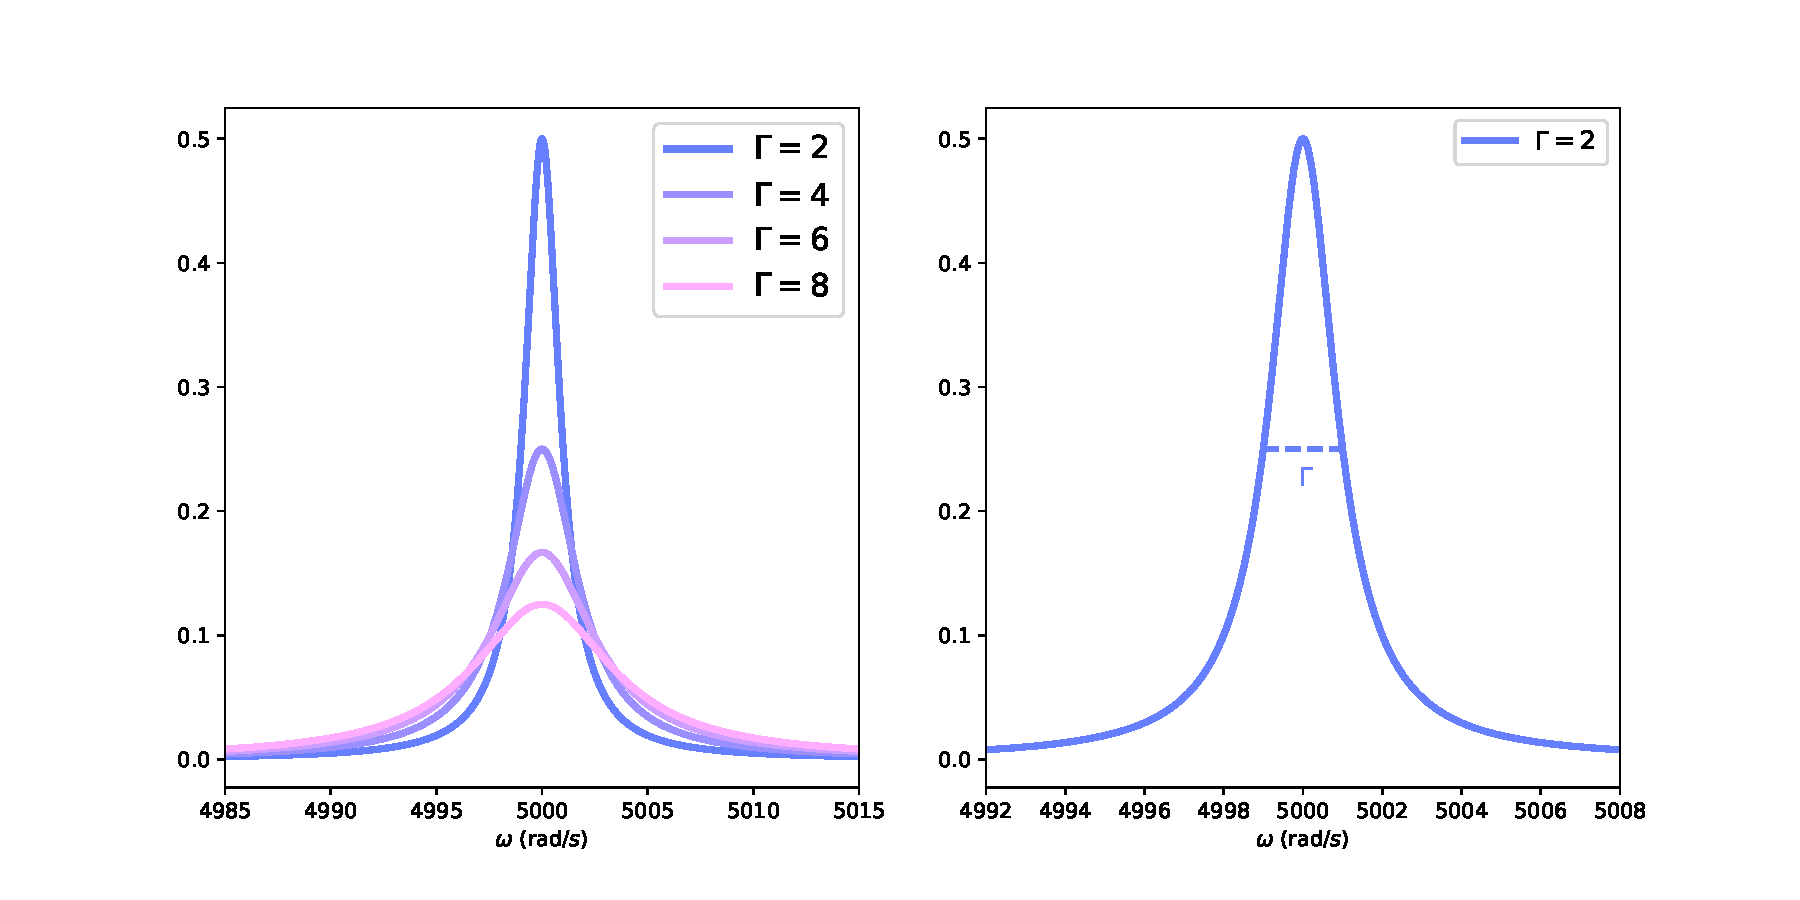
\includegraphics[scale=0.57]{Seccion.pdf}
\caption{sección eficaz de absorción en función de la frecuencia para $\omega_0$= 5000 rad/s.}
\label{Fig:7.3.02}
\end{figure}

Sea un medio con una cantidad $N$ de osciladores por unidad de volumen $N$. Si consideramos una onda de frecuencia bien definida $\omega$ que se desplaza una cantidad diferencial $\D z$ a lo largo del eje z, considerando una sección transversal de área $S$ el número de osciladores irradiando es $\D n = N S \D z$, ya que $\D n / \D V = N$. Considerando que cada oscilador absorbe una potencia, tendremos que la energía perdida es:

\begin{equation}
\D P = - P \D n = - \sigma I S N \D z
\end{equation}
tal que si dividimos por el área $S$ esta ecuación corresponde a una variación de la irradiancia, como se puede ver en la siguiente ecuación:

\begin{equation}
\dfrac{\D P}{S} = \D I = - \sigma I N \D z
\end{equation}
que lleva irremediablemente a que:

\begin{equation}
I(z)=I_0 e^{-\alpha z}
\end{equation}
Esta ecuación donde $\alpha=\sigma N$ es conocida como la \textit{ley de Bouger} o \textit{ley de Beer-Lambert}. Segunda esta ley, la irradiancia decrece exponencialmente con la distancia propagada. La caída será mas grande cuanto mayor sea $\sigma$ o cuando mayor sea $N$. Para una frecuencia dada $\alpha$ es una característica del material, que puede variar drasticamente. 

\subsection{Dispersión de Rayleigh}

Un medio trasparente es aquel medio cuya irradiancia no cae, es decir, es todo medio donde $\sigma \rightarrow 0$. Esto se puede entender como que $|\omega  - \omega_0| \gg \Gamma$. En ese claro esta claro que:

\begin{equation}
x(t) = \dfrac{e}{m} \dfrac{1}{\omega^2 - \omega_0^2} |A| \cos (\omega t - \delta)
\end{equation}

En gran parte de los casos la zona de la frecuencia de resonancia se encuentra en el espectro de los rayos UV, de tal modo que si estudiamos ondas de la frecuencia de la luz visible, dicha frecuencia será despreciable frente la frecuencia de resonancia, y por tanto:

\begin{equation}
x(t) = x_0 \cos(\omega t - \delta) \tquad x_0 = - \dfrac{e}{m} \dfrac{1}{\omega_0^2} |A|
\end{equation}

Que no es otra cosa que un \textit{dipolo oscilante} tal y como vimos en el apartado  \ref{Subsub:7.2.1}. Es entonces aplicable todas las expresiones vistas pero ahora en vez de oscilar con su frecuencia de resonancia $\omega_0$ (que es lo que haría si no hubiera un campo externo) el dipolo oscilará con $\omega$. La irradiancia $I_r$ que reemite, y repito, que \textit{reemite}, viene dada por la ecuación \ref{Ec:7.2.1.08}. Dado que en este caso $x_0 = e |A| /m \omega_0^2$ tendremos que:

\begin{equation}
I_r = \dfrac{e^4 \omega^4 |A|^2}{32 m^2 \pi^2 \varepsilon_0 c^3 \omega_0^4} \dfrac{\sin^2 \theta}{R^2}
\end{equation}
que si integramos en una superficie esférica obtendremos la potencia total reemitida por el dipolo eléctrico, que viene dada por:

\begin{equation}
P_r = \dfrac{e^4 \omega^4 |A|^2}{12 \pi m^2 \varepsilon_0	c^3 \omega_0^4}
\end{equation}

Estas expresiones se relacionan directamente con la irradiancia de la onda, ya que si $E=A \cos(\omega t)$, podemos ver que $I=\varepsilon_0 c |A|^2 / 2$ es la irradiancia de la onda. Podemos definir la potencia reemitida en función de la irradiancia de la onda que llega, tal que:

\begin{equation}
P_r = \dfrac{e^4 \omega^4}{6 \pi m^2 \varepsilon_0^2 c^4 \omega_0^4} I
\end{equation}

Este resultado obtenido para la reemisión de la energía por un \textit{único} oscilador atómico se puede generalizar a un medio, siempre que las partículas estén bien separadas. En ese caso podemos considerar un modelo de partículas independientes, y la potencia reemitida como la suma de todas las potencias dispersadas por cada uno de los átomos/moléculas. A este tipo de dispersión se le conoce como \textbf{dispersión de Rayleigh}, y es responsable de que el cielo sea de color azul la mayor parte del día y naranja/rojo en el horizonte en el atardecer. \\

\subsection{Modelo simple del índice de refracción}

Podemos usar el conocimiento adquirido para estudiar el índice de refracción en un medio trasparente (no hay absorción) homogéneo. Consideremos que la velocidad de fase es menor que la velocidad de la luz, donde hay una relación dada por un factor $n$:

\begin{equation}
v = \dfrac{c}{n}
\end{equation}

Llamaremos a este factor $n$ la \textbf{refracción del medio} para la frecuencia $ \omega$, como podíamos intuir. En ese caso la onda monocromática que llega al medio (que se propaga en el eje z) vendrá dada por:

\begin{equation}
E = A e^{i (kz-\omega t)}
\end{equation}
donde $k = n k_0 = n \omega/c = k_0 + (n-1) k_0$. Es decir, la onda vendrá dada por:

\begin{equation}
E = A e^{i (k_0z-\omega t} e^{i (n-1)k_0 z} \label{Ec:7.5.0.31}
\end{equation}
expresado de esta forma podemos ver que la onda en dicho medio se comporta como una onda en el vacío desfasada un factor $(n-1)k_0 z$. Entonces en una distancia $\Delta z$ la onda en dicho medio se desfasará un $\Delta \varphi$ respecto la del vacío 

\begin{equation}
\Delta \varphi = (n-1)k_0 \Delta z
\end{equation}

Si desarrollamos el complejo desfase de la ecuación \ref{Ec:7.5.0.31} y aproximamos por taylor el coseno y seno (para hacer esto hay que considerar que $n \approx 1$) tal que:

\begin{equation}
E=A e^{i (k_0z-\omega t)}  ( \cos (\Delta \varphi) + i  \sin (\Delta \varphi) ) \longrightarrow E = A e^{i (k_0z-\omega t)}  (	1+ i\Delta \varphi )
\end{equation}

Consecuentemente podemos entender la propagación de una onda por dicho medio (siempre que $n \approx 1$) como la suma de una onda que se propaga por el vacío mas 
otra mas débil desfasada $\pi/2$ respecto esta. Ahora vamos a ver como podemos relacionar todo esto con el desfase producido por un \textit{dipolo oscilante} en un medio homogéneo. \\

Sabemos que un dipolo oscilante en presencia de un campo eléctrico incidente radia un campo eléctrico secundario, denominado $E_{\mathrm{dip}}$. Si la oscilación es:

\begin{equation}
x = x_0 e^{i (\omega t + \delta)} \tquad x_0 = \dfrac{e}{m} \dfrac{1}{\omega^2-\omega_0^2} A
\end{equation}
donde $A \in \mathbb{C}$, tendremos que el campo eléctrico generado por el dipolo será:
\begin{equation}
E_{\mathrm{dip}} = \dfrac{e \omega^2 x_0}{8 \pi \varepsilon_0 c^2} \dfrac{\sin \theta}{R} e^{-i \omega (t - R/c)}
\end{equation}

Ahora bien, esto es el campo generado por \textit{un solo oscilador}, en el medio hay muchísimos osciladores, considerando, como antes que hay un número $N$ de osciladores por unidad de volumen. Vamos a calcular entonces la superposición de la emisión dipolar en una lámina fina de espesor $\Delta z$ en un punto $P$ situado a una distancia de la lámina mucho mayor que el espesor (centrada respecto a este). En ese caso podremos considerar que todos los dipolos (desde el punto de vista de $P$) que todos los dipolos están situados en el mismo plano, situados en diferentes puntos del plano, tal que $R$ es diferente. Suponemos ahora coordendas cilíndricas donde $\rho$ te da la distancia entre el centro de la lámina al oscilador y $\varphi$ el ángulo respecto al eje x que esta situado. Entonces el campo dipolar (que expresamos como $E_{ad}$) resultante en toda la lámina será:


\begin{equation}
\D E_{ad} = E_{dip} \D n = E_{dip} N \Delta z \rho \D \rho \D \varphi
\end{equation}
y por tanto

\begin{equation}
E_{\mathrm{ad}} = \dfrac{e x_0 \omega^2}{8 \pi \varepsilon_0 c^2} N \Delta z e^{i \omega t} \int \dfrac{\sin \theta}{R} e^{i k_0 R} \rho \D \rho \D \varphi
\end{equation} 
dado que $z \gg \rho$ tendremos que $R = \sqrt{z^2 + \rho^2} \approx z(1+\frac{\rho^2}{2z^2}) = z + \rho^2 / 2 z$. En ese caso la integral anterior tendrá la siguiente solución, bastante difícil de encontrar ya que existe una relación de $\theta$ con $\varphi$. De cualquier forma si llamamos $K$ al resultado de dicha integral, el campo vendrá dado por:

\begin{equation}
E_{ad} = - i \dfrac{N e^2}{8 \varepsilon_0 m \omega^2} \dfrac{K}{\omega^2 - \omega_0^2} k_0 \Delta z E_{in}
\end{equation}

Dicho esto queda claro que si $E=E_{in}+E_{ad}$ donde $E_{in}$ es el campo propagándose por el vacío podremos asociar claramente $n$ con el resto de factores:

\begin{equation}
n = 1 -   \dfrac{N e^2}{8 \varepsilon_0 m} \dfrac{K}{\omega^2 - \omega_0^2} \label{Ec:7.5.0.38}
\end{equation}

En función de la configuración espacial de los átomos/moléculas y otros parámetros microscópicos obtendremos un valor de $K$ u otro. 


\subsubsection{Oscilador no lineal}

El oscilador no lineal es un oscilador que no tiene porque tener un movimiento armónico, i.e. no tienen una fuerza de ``retorno'' del tipo $-\frac{\omega_0}{k}x$. Para describir esto lo que hacemos es usar una fuerza genérica $U(x)$ proveniente de un potencial, tal que:

\begin{equation}
\ddot{x} + \Gamma \dot{x} + \dfrac{U(x)}{m} = - \dfrac{e}{m}M 
\end{equation}


 \newpage

\section{Dispersión material e índice complejo}

Como ya hemos dicho muchos materiales presentan frecuencias de resonancia en el rango de los UV, pero también presentan resonancia con otras frecuencias, como puede ser la molécula de agua en el caso de las ondas de microondas. En este tema veremos como podemos representar esto en el marco de la óptica electromagnética usando índices de refracción complejos. Como hemos visto podemos representar el comportamiento de las ondas en medio con conductividad con un índice de refracción complejo. Aunque no lo hemos visto, en realidad los medios dieléctricos también pueden describirse con índices de refracción complejos, siempre que haya un desfase entre polarización y campo eléctrico. Como sabemos:

\begin{equation}
\Pn = \varepsilon_0 \chi \En \label{Ec:8.0.0.01}
\end{equation}
tal que el índice de refracción viene dado por:

\begin{equation}
n = \sqrt{1+\chi}
\end{equation}

Podemos relacionar las magnitudes polarización $\Pn$ y flujo eléctrico $\Jn$ con cantidades microscópicas usando la cantidad de átomos/moléculas por unidad de volumen, tal que:

\begin{equation}
\Pn = N \pn \tquad \Jn = \rho \vn \label{Ec:8.0.0.04}
\end{equation}

\subsection{Dispersión en dieléctricos}

Vamos a usar ahora el modelo de Lorentz, usado en el tema anterior para analizar la \textit{dispersión de Rayleigh}, usando como modelo un gas a baja presión, con átomos/moléculas separados a la suficiente distancia para poder despreciar la interacción mutua, de tal manera que solo actúa sobre ellos la fuerza electromagnética. \\

Como sabemos la polarización se relaciona con el campo eléctrico mediante una constante llamada susceptibilidad eléctrica. Lo mismo ocurre con el dipolo eléctrico, tal que:

\begin{equation}
\pn = \alpha_p \En
\end{equation}
donde $\alpha_p$ es la \textit{polarizabilidad}, que viene dada por (usando \ref{Ec:8.0.0.04}):

\begin{equation}
\alpha_p = - \dfrac{e^2}{m} \dfrac{N}{\omega^2 - \omega_0^2 + i \omega \Gamma} \label{Ec:8.1.0.05}
\end{equation}
Ahora bien, ¿De donde sale esto? Pues de unir las ecuaciones \ref{Ec:7.1.0.02}, \ref{Ec:7.3.0.12}. Si relacionamos la ecuación anterior (\ref{Ec:8.1.0.05}) con la  ecuación \ref{Ec:8.0.0.01} vemos claramente que:

\begin{equation}
\varepsilon_0 \chi = \alpha_p
\end{equation}
y por tanto:

\begin{equation}
n^2_c = 1 - \dfrac{N e^2}{\varepsilon_0 m} \dfrac{1}{\omega^2 - \omega^2_0 + i \omega \Gamma} \label{Ec:8.1.0.07}
\end{equation}
Es común escribir $\omega_p$ al factor que acompaña al cociente complejo. Realmente no nos importa el complejo del número complejo, nos importa el número complejo. Si consideramos que $n \approx 1$, entonces podemos usar el desarrollo de Taylor para describir el índice complejo, de tal manera que:

\begin{equation}
n_c = n + i \kappa \simeq 1 - \dfrac{1}{2} \dfrac{\omega_p^2}{\omega^2 - \omega_0^2 + i \omega \Gamma}
\end{equation}
Separando la parte real y la parte imaginaria obtenemos que:

\begin{equation}
n = 1 - \dfrac{\omega_p^2 (\omega^2-\omega_0^2)}{(\omega^2-\omega_0^2)^2 + (\omega \Gamma)^2} \tquad \kappa = \dfrac{1}{2} \dfrac{\omega \Gamma \omega_p^2}{(\omega^2 - \omega_0^2)^2 + (\omega \Gamma)^2}
\end{equation}



\begin{figure}[h!] \centering
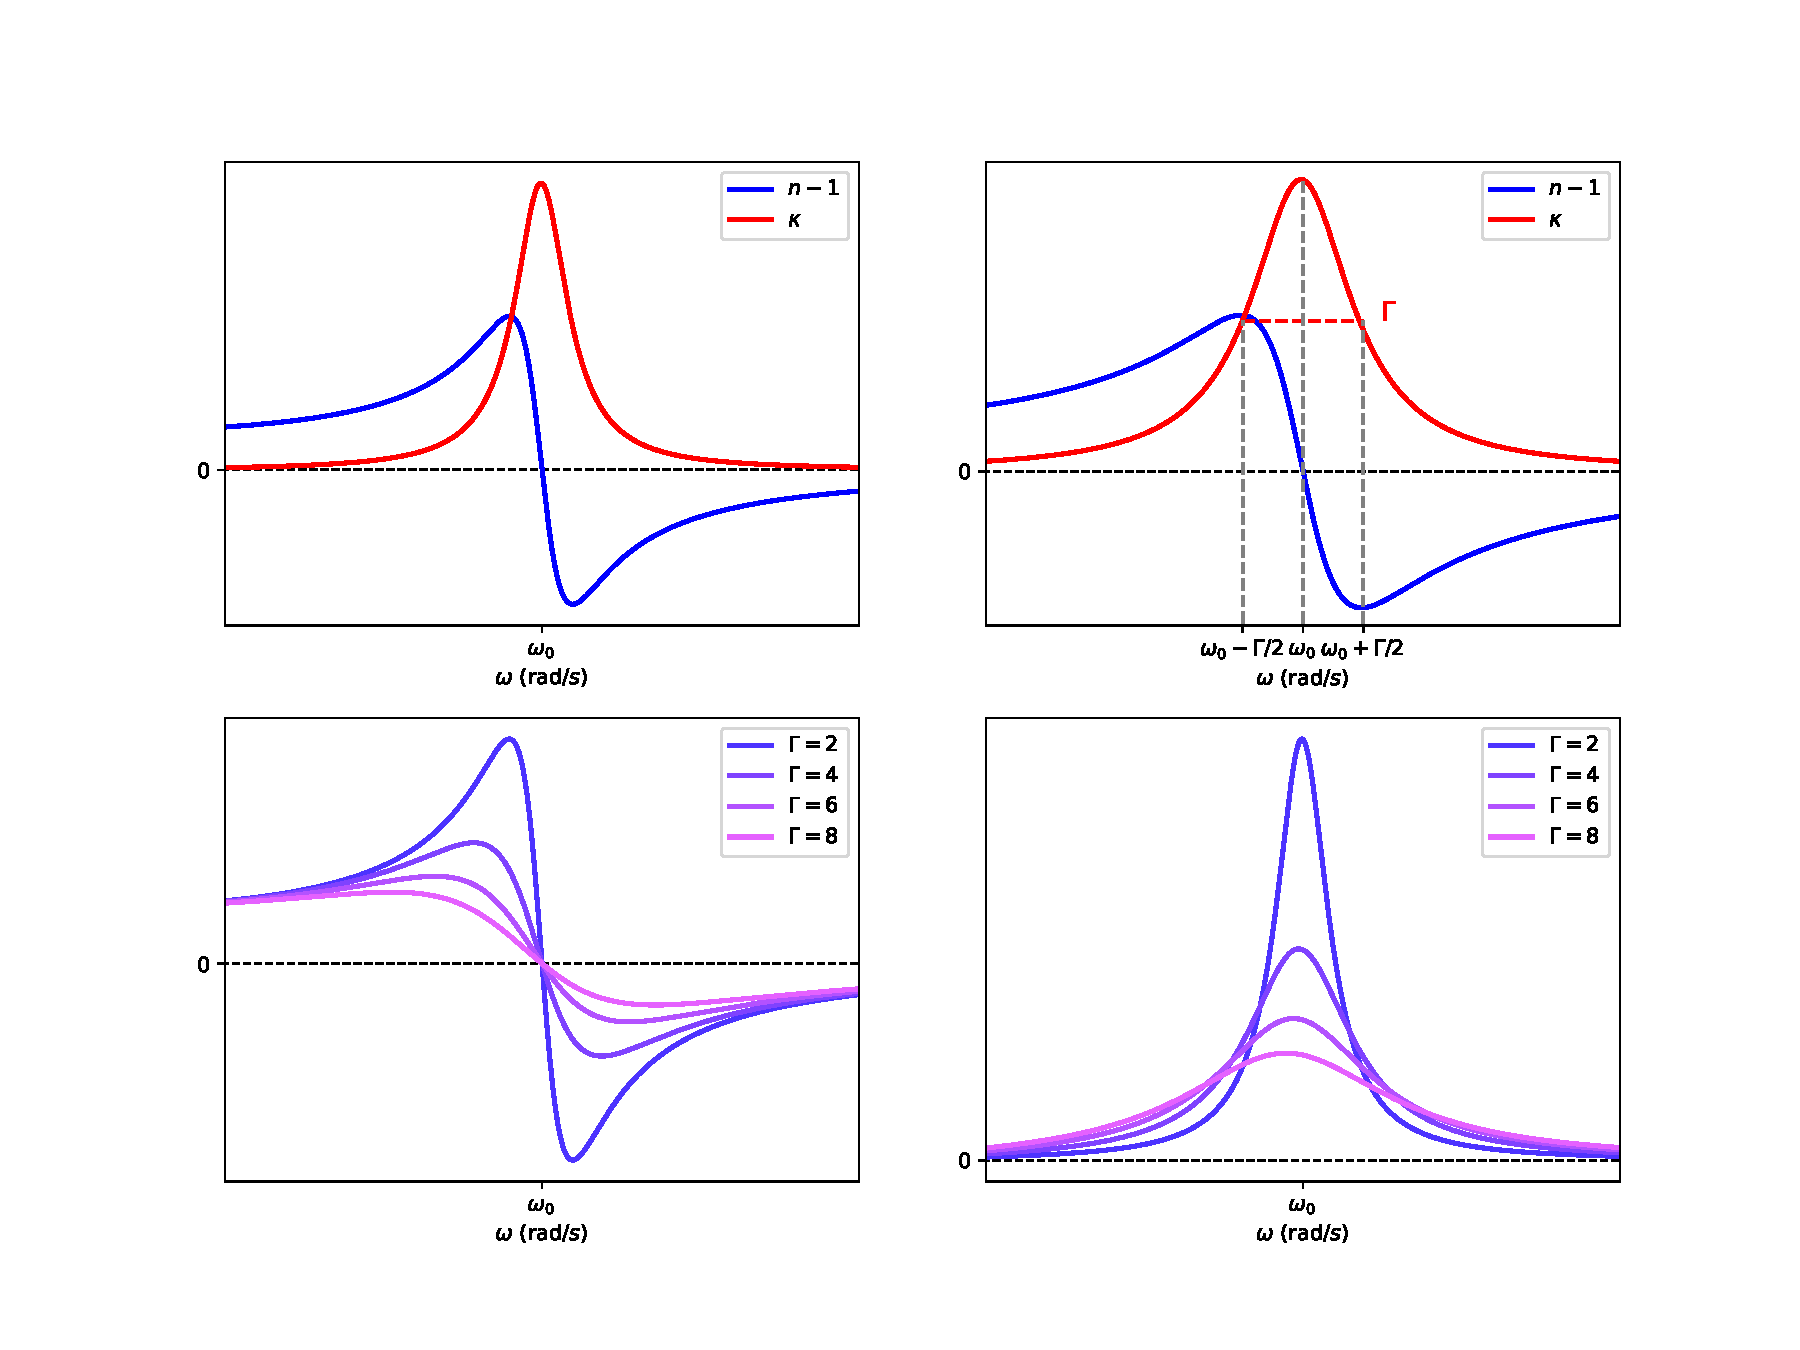
\includegraphics[scale=0.55]{indicecomplejo.pdf}
\caption{diferentes gráficas para el índice complejo.}
\label{Fig:8.1.01}
\end{figure}


En la figura \ref{Fig:8.1.01} podemos observar diferentes gráficas para el índice complejo, representando de manera separa el comportamiento de la parte real y la parte imaginaria según la frecuencia y la tendencia según $\Gamma$. Podemos ver como la parte imaginaria tiene un máximo en la frecuencia de resonancia, tal y como cabría esperar. \\

En una dispersión normal, sin ningún tipo de absorción el número complejo sería un número puramente real $\Gamma=0$. En ese caso la expresión del índice de refracción sería muchísimo mas simple, dado por:

\begin{equation}
n^2 = 1 -  \dfrac{\omega_p^2}{\omega^2-\omega^2_0}
\end{equation}

Podemos comparar esta expresión del índice de refracción con la ecuación \ref{Ec:7.5.0.38}. Es decir el modelo de la lamina fina y el modelo para un índice complejo son equivalentes si $K=4$. \\

Sin embargo como hemos dicho antes gran parte de los materiales tiene \textit{varias frecuencias de resonancia}. ¿Como se modela esto? Considerando que hay diferentes tipos de osciladores, con diferentes frecuencias propias, constantes de amortiguamiento y densidades. En ese caso la constante  dieléctrica compleja puede obtenerse como la suma de susceptibilidades eléctricas, tal que:

\begin{equation}
n_c = 1 - \dfrac{e^2}{\varepsilon_0 m} \sum_j \dfrac{N_j}{\omega^2 - \omega^2_j + i \omega \Gamma}
\end{equation}

\subsubsection{Dieléctricos densos}

En los gases con una presión normal, en cualquier líquido o sólido estas aproximaciones realizadas no son válidas, por lo que el índice de refracción deja de ser parecido a 1. La razón es que cada oscilador no solo se ve afectado por el campo incidente, si no que se ve afectado por el campo reemitido por cada oscilador. El efecto resultante es que la fuerza eléctrica que actúa sobre un dipolo difiere de la ejercida por el campo exterior $\En$. Para resolver este problema introducimos un campo local $\En_i$ que incluye el efecto de los osciladores mas cercanos, tal que:

\begin{equation}
\pn = \alpha_p \En
\end{equation}

El propio Lorentz al estudiar diferentes materiales ya encontró un valor \textit{experimental} para medios opticamente isótropos asumiendo una simetría esférica. Este valor viene dado por:

\begin{equation}
\En_i = \En + \Pn /3 \varepsilon_0
\end{equation}
En este caso combinando todas las ecuaciones podemos llegar a  que el índice complejo viene dado por:

\begin{equation}
n_c^2 = 1 + \dfrac{N \alpha_p}{\varepsilon_0 - N \alpha_p/3}
\end{equation}
que se suele expresar usando la \textit{ecuación de Claussius-Mossotti} también llamada ecuación de \textit{Lorentz-Lorenz}:

\begin{equation}
\dfrac{n_c^2 - 1}{n_c^2 + 2} = \dfrac{N \alpha_p}{3 \varepsilon_0}
\end{equation}

En una situación realista tendremos que tener en cuenta las diferentes resonancias de los medios y suma de polarizabildades, pesadas por diferentes densidades $N_j$. Para cada resonancia tendremos una banda de absorción con dispersión anómala.

\subsection{Dispersión en medios conductores}

En los medios conductores debemos tener en cuenta la conductividad del material asociada al movimiento de las cargas libres. Para tener en cuenta modificaremos el modelo de Loretnz previamente estudiado, suponiendo que \textit{no existe fuerza de restauración}, i.e. no se comporta como un oscilador armónico. Entonces la ecuación del movimiento:

\begin{equation}
\ddot{\rn} + \Gamma \dot{\rn} = - e \En / m \tquad \dot{\vn} + \Gamma \vn = - e \En / m
\end{equation}

En esta ecuación no consideramos el efecto de la interacción del electrón con átomos cercanos, ya que el electrón tiene gran mobilidad y no está localizado. Por otro lado, el valor de la constante de amortiguamiento viene afectada por las colisiones con los iones positivos, por lo que es mas grande. Si consideramos una onda incidente monocromáticai  $\En = \An e^{i \omega t}$:

\begin{equation}
\vn = \vn_0 e^{-i \omega t} \tquad \vn_0 = \dfrac{e \An}{m} \dfrac{1}{i \omega - \Gamma}
\end{equation}

Con esta relación y la ecuación \ref{Ec:8.0.0.04} podemos obtener el valor de la corriente de cargas, tal que $\Jn = - N e \vn$, donde $N$ es la \textit{densidad de electrones libres}. En este caso podremos obtener que la conductividad es:

\begin{equation}
\sigma_c = \dfrac{N e^2}{m} \dfrac{1}{\Gamma-i \omega}
\end{equation}

Tal que el índice complejo dado por $n_c^2 = 1+ \sigma_c/\varepsilon_0 \omega$ (donde asumimos que el efecto de la carga ligada es despreciable y por tanto $\varepsilon_r = 1$) se podrá expresar como:

\begin{equation}
n_c = \sqrt{1+\dfrac{\omega_p^2}{\omega^2+ i \Gamma \omega}}
\end{equation}
que es completamente equivalente a la expresión obtenida en \ref{Ec:8.1.0.07} si suponemos que no hay frecuencia de resonancia. Es entonces claro que si $\omega \ll \Gamma$ (caso metales) tendremos que:

\begin{equation}
n_c \simeq \sqrt{i \dfrac{\omega^2_p}{\Gamma \omega}} \longrightarrow n \simeq \kappa \simeq \sqrt{\dfrac{\sigma_0}{\varepsilon_0 \omega}}
\end{equation}
donde hemos supuesto también que $\omega_p^2 \gg \omega \Gamma$ y por tanto el factor uno despreciable. Si la aproximación es que $\Gamma \ll \omega$ (caso de gases ionizados) tendremos que:

\begin{equation}
n_C = n = \sqrt{1-\dfrac{\omega^2_p}{\omega^2}}
\end{equation}
que muestra que para frecuencias menores que la frecuencia $\omega_p$ también llamada \textit{frecuencia de plasma} el índice de refración es completamente imaginario: medio completamente opaco a la radiación.

\newpage

\section{Polarización}

\subsection{Introducción}

Cuando estudiemos la propagación de ondas planas hemos visto que los campos eléctrico y magnético son completamente trasversales a la dirección de propagación. Es decir, están restringidas en un plano cuya dirección de propagación es la normal a dicho vector. La \textbf{polarización} de la luz habla de como vibran los campos eléctromagnéticos en dicho plano. \\

En las expresiones de los temas anteriores hemos supuesto que el campo magnético y eléctrico siempre mantenían una misma dirección de vibración, pero esto no es siempre cierto: pueden variar con el tiempo. En este tema vamos a estudiar las 3 polarizaciones: lineal, circular y elíptica.

\subsection{Polarización en medios isótropos}

Para fijar ideas vamos a considerar ondas planas monocromáticas que se propagan en el eje $z$. Aunque cuando estudiemos la polarización normalmente nos fijamos en la forma del campo eléctrico, ya que la ecuación del campo magnético vendrá determinada por $\Bn = \frac{1}{\omega} \kn \times \En$.  \\

Si $\sn = \hnz$, para que $\En$ sea perpendicular tiene que vivir en el plano $XY$, y por tanto solo puede tener componentes en el eje $x$ y en el eje $y$. Para cualquier problema con estas características se verificará que

\begin{equation}
\En = E_x \hnx + E_y \hny
\end{equation}
donde $E_x$ y $E_y$ son números complejos. Podemos suponer entonces que la diferencia entre las componentes $E_x$ y $E_y$ vendrán dadas únicamente por un módulo y un desfase, que podemos representar como:

\begin{equation}
E_x = A_x \cos (kz-\omega t + \varphi_x) \tquad E_y = A_y \cos (kz - \omega t + \varphi_y)
\end{equation}
donde suponemos que amplitudes son positivas. Una fase global no afecta a una onda monocromática, por lo que es común suponer que $A_x$ no tiene desfase y todo el desfase se acumula en la componente $y$. De esta forma la componente $y$ acumula toda la desfase entre $x$ e $y$ y por tanto toda la información del desfase entre componentes. Expresado de manera compleja:

\begin{equation}
\En = ( A_x \hnx +  A_y e^{\Delta \varphi} \hny) e^{i (kz - \omega t)} \label{Ec:09.2.0.03}
\end{equation}
donde el campo será la parte real de dicho número complejo, y $\Delta \varphi = \varphi_y - \varphi_y$.

\subsubsection{Polarización lineal}

La polarización lineal es el tipo de polarización que hemos estudiado en los temas anteriores: los campos vibran siempre en la misma dirección del movimiento:


\begin{equation}
 \En = (A_x \hnx \pm  A_y \hny) \cos (kz-\omega t)
\end{equation}

Si lo comparamos con la expresión \ref{Ec:09.2.0.03} podemos ver claramente que el signo vendrá determinado para dos desfases muy concretos: si $+$ tenemos que $\Delta \varphi = 0$ y si $-$ tenemos que $\Delta \varphi = \pi$. Como resultado el campo vibra en una dirección formando un ángulo con el eje $x$ dado por:

\begin{equation}
\tan \theta = \pm \dfrac{A_x}{A_y}
\end{equation}
Siguiendo la notación complejo la luz linealmente polarizada puede expresarse como:

\begin{equation}
 \En = (A_x \hnx  \pm A_y \hny) e^{i (kz-\omega t)}
\end{equation}

En la figura \ref{Fig:9.2.1.01} se puede observar que una onda polarizada en una dirección del espacio concreto puede entenderse como la suma de una onda linealmente polarizada en el eje $x$ y otra en el eje $y$ \textit{siempre que esten en fase total o en desfase total}.

\begin{figure}[h!] \centering
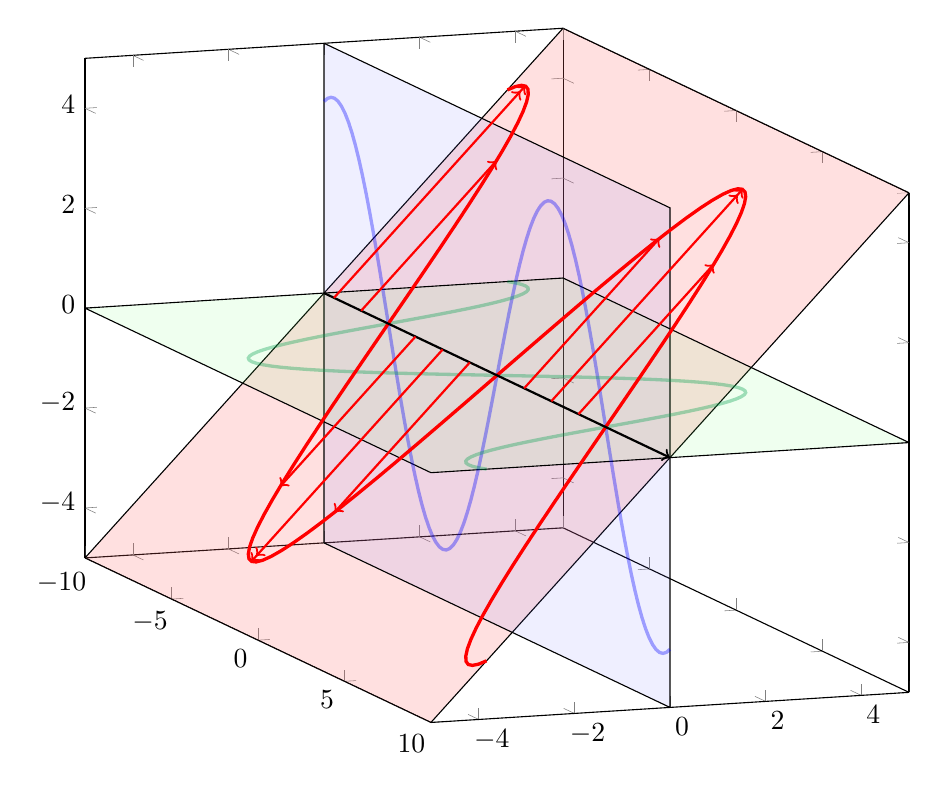
\begin{tikzpicture}
\begin{axis}[xmax=10,ymax=5,xmin=-10,ymin=-5,zmax=5,zmin=-5,view={70}{10},plot box ratio=2 1 1,
]
\addplot3 [fill=red!60,fill opacity=0.2] coordinates {(-10,-5,-5)(10,-5,-5)(10,5,5)(-10,5,5)(-10,-5,-5)} \closedcycle;
\addplot3 [fill=blue!60,fill opacity=0.1] coordinates {(-10,0,-5)(-10,0,5)(10,0,5)(10,0,-5)(-10,0,-5)} \closedcycle;
\addplot3 [fill=green!60,fill opacity=0.1] coordinates {(-10,-5,0)(-10,5,0)(10,5,0)(10,-5,0)} \closedcycle;

\addplot3+[blue,no markers,samples=100, samples y=0,domain=-10:10,variable=\t,style={very thick},opacity=0.35] ({\t},{0},{4*sin(\t/2 r)});
\addplot3+[color1,no markers,samples=100, samples y=0,domain=-10:10,variable=\t,style={very thick},opacity=0.35] ({\t},{4*sin(\t/2 r)},{0});
\addplot3+[red,no markers,samples=100, samples y=0,domain=-10:10,variable=\t,style={very thick,solid}] ({\t},{4*sin(\t/2 r)},{4*sin(\t/2 r)});
\addplot3+[black,no markers,samples=5, samples y=0,domain=-10:10,variable=\t,style={thick,solid},->] ({\t},{0},{0});

\addplot3+[red,no markers,samples=51, samples y=0,domain=0:4),variable=\t,style={thick,solid},->>] ({pi},{\t},{\t});
\addplot3+[red,no markers,samples=51, samples y=0,domain=0:(4),variable=\t,style={thick,solid},->>] ({-pi},{-\t},{-\t});
\addplot3+[red,no markers,samples=51, samples y=0,domain=0:4,variable=\t,style={thick,solid},->>] ({-3*pi},{\t},{\t});                                                                

\addplot3+[red,no markers,samples=51, samples y=0,domain=0:4*sin(pi/4 r),variable=\t,style={thick,solid},->] ({-3*pi/2},{-\t},{-\t});                                                                
\addplot3+[red,no markers,samples=51, samples y=0,domain=0:4*sin(pi/4 r),variable=\t,style={thick,solid},->] ({-pi/2},{-\t},{-\t});                                                                

\addplot3+[red,no markers,samples=51, samples y=0,domain=0:4*sin(pi/4 r),variable=\t,style={thick,solid},->] ({3*pi/2},{\t},{\t});                                                                
\addplot3+[red,no markers,samples=51, samples y=0,domain=0:4*sin(pi/4 r),variable=\t,style={thick,solid},->] ({pi/2},{\t},{\t});                                                                

\addplot3+[red,no markers,samples=51, samples y=0,domain=0:4*sin(pi/4 r),variable=\t,style={thick,solid},->] ({-5*pi/2},{\t},{\t});                                                                
\end{axis}
\end{tikzpicture}
\caption{luz linealmente polarizada propagandose en el eje z}
\label{Fig:9.2.1.01}
\end{figure}

\subsubsection{Polarización circular}

La polarización circular es un caso muy concreto del último tipo de polarización: la polarización elíptica. De hecho la polarización lineal es también un caso de la polarización elíptica.  \\

La polarización circular debe cumplir dos condiciones: el desfase es de $\pm \pi/2$ y que $A\equiv A_x=A_y$. En cualquier caso tendremos polarización elíptica. Es decir el campo viene dado por:

\begin{equation}
\En(x,t) = A (\hnx \cos(kz-\omega t) \pm \hny \sin (kz-\omega t))  \quad \dot{\En} (x,t) = A (\hnx \sin (kz-\omega t) \mp \cos (kz-\omega t)) \label{Ec:09.2.2.07}
\end{equation}
o si lo escribimos en números complejos:

\begin{equation}
\En = A(\hnx \mp i\hny) e^{i (kz-\omega t)} \tquad \dot{\En} = A ( i \hnx \pm \hny) e^{i (kz-\omega t)} \label{Ec:09.2.2.08}
\end{equation}
donde ponemos $\mp$ ya que si en la parte real va con $+$ debido al cambio de signos por el producto de imaginarios debemos tener un $-$ en la forma imaginaria. \\

En la figura \ref{Fig:9.2.2.02} podemos ver claramente que es la polarización circular. Como podemos ver el campo eléctrico apunta hacia un sitio diferente en función de la posición de $z$. El campo eléctrico al propagarse apunta a sitios diferentes. Sin embargo no debemos pensar que siempre apunta al mismo sitio: la imagen está hecha para un instante $t_0$ concreto. Si estudiamos el comportamiento de la onda en un punto $z$ cualquiera a lo largo del tiempo podremos ver que este también cambia de posición describiendo un círculo.


\begin{figure}[h!] \centering
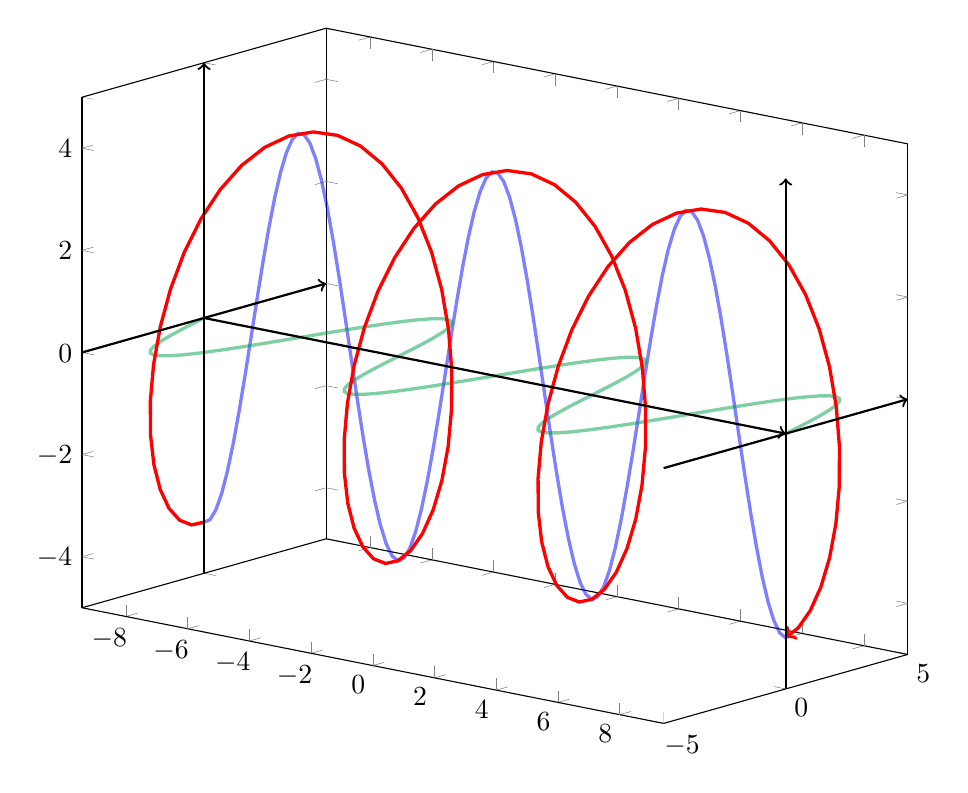
\begin{tikzpicture}
\begin{axis}[xmax=3*pi,ymax=5,xmin=-3*pi,ymin=-5,zmax=5,zmin=-5,view={40}{10},plot box ratio=2 1 1,
]


\addplot3+[blue,no markers,samples=100, samples y=0,domain=-3*pi:3*pi,variable=\t,style={very thick},opacity=0.5] ({\t},{0},{4*cos(\t r)});
\addplot3+[color1,no markers,samples=100, samples y=0,domain=-3*pi:3*pi,variable=\t,style={very thick},opacity=0.5] ({\t},{4*sin(\t r)},{0});
\addplot3+[red,no markers,samples=100, samples y=0,domain=-3*pi:3*pi,variable=\t,style={very thick},opacity=1,->] ({\t},{4*sin(\t r)},{4*cos(\t r)});

\addplot3+[black,no markers,samples=5, samples y=0,domain=-3*pi:3*pi,variable=\t,style={ thick,solid},->] ({\t},{0},{0});


\addplot3+[black,no markers,samples=100, samples y=0,domain=-5:5,variable=\t,style={ thick,solid},->] ({-3*pi},{\t},{0});
\addplot3+[black,no markers,samples=100, samples y=0,domain=-5:5,variable=\t,style={ thick,solid},->] ({3*pi},{\t},{0});

\addplot3+[black,no markers,samples=100, samples y=0,domain=-5:5,variable=\t,style={ thick,solid},->] ({-3*pi},{0},{\t});
\addplot3+[black,no markers,samples=100, samples y=0,domain=-5:5,variable=\t,style={ thick,solid},->] ({3*pi},{0},{\t});


%\addplot3+[black,no markers,samples=100, samples y=0,domain=-5:5,variable=\t,style={ thick}] ({3*pi},{-5},{\t});
%\addplot3+[black,no markers,samples=100, samples y=0,domain=-5:5,variable=\t,style={ thick}] ({3*pi},{\t},{5});
%\addplot3+[black,no markers,samples=5, samples y=0,domain=-3*pi:3*pi,variable=\t,style={ thick}] ({\t},{-5},{5});
\end{axis}

\end{tikzpicture}
\caption{luz circularmente polarizada propagándose en el eje z}
\label{Fig:9.2.2.02}
\end{figure}

Otro factor muy importante a la hora de estudiar las ondas de polarización circular (y elíptica) es el estudio de la \textbf{onda levógira} o \textbf{onda dextrógira}. Una onda dextrógira o también llamada onda \textit{a derechas} es aquella que verifica $+$ para la expresión real (\ref{Ec:09.2.2.07}) o $-$ para la expresión compleja (\ref{Ec:09.2.2.08}). Una onda levógira también llamada onda \textit{a izquierdas} verifica $-$ para la expresión real (\ref{Ec:09.2.2.07})  o $+$ para la expresión compleja (\ref{Ec:09.2.2.08}). \\

Para estudiar esto lo que vamos hacer es crear un ``momento angular'' que nos hable en todo momento de la posición de la onda en el círculo y hacia donde se dirige, tal que $\rn =\frac{1}{\sqrt{2}} (\hnx \mp i \hny)$ y obviamente $\vn = \frac{1}{\sqrt{2}} \omega(i \hnx \pm \hny)$ (estando los vectores unitarios normalizados), tal que: 

$$ \Ln  \equiv \rn \times \vn = \frac{1}{2} \omega (\hnx \mp i \hny ) \times (i \hnx \mp \hny) = \pm \omega \hnz $$
y por tanto tendremos que:

\begin{equation}
\Ln = \pm \omega \hnz
\end{equation}
como podemos ver claramente $\Ln$ solo puede tener dos direcciones: \textit{paralela} a la dirección de propagación y \textit{antiparalela} a la dirección de propagación, de tala modo que el \textit{paralelo} es equivalente al \textit{dextrógiro} y que el \textit{antiparalelo} es equivalente al \textit{levógiro}. Cuando cogemos el $-$ en el complejo vemos que $\Ln = \omega \hnz$ y por tanto dextrógiro; si cogemos el $+$ en el complejo vemos que $\Ln = - \omega \hnz$ y por tanto levógiro.


\subsubsection{Polarización elíptica}

La polarización elíptica como hemos mencionado es el caso mas general, donde el campo viene dado por la parte real de la siguiente ecuación

\begin{equation}
\En = (A_x\hnx+A_y e^{i \Delta \varphi}\hny) e^{i (kz-\omega t)}
\end{equation}

La única condición que debe verificarse para poder hablar de polarizaciçon elíptica es que el desfase debe ser el mismo para todo $t$ y $z$, algo que no se cumple por ejemplo con una lámina retardadora. Como podemos ver los dos casos anteriores están incluidos en este caso. En el caso de la polarización elíptica mantendremos las propiedades levógiras y dextrógiras, calculándose de manera completamente análoga a la circular.
\begin{figure}[h!] \centering
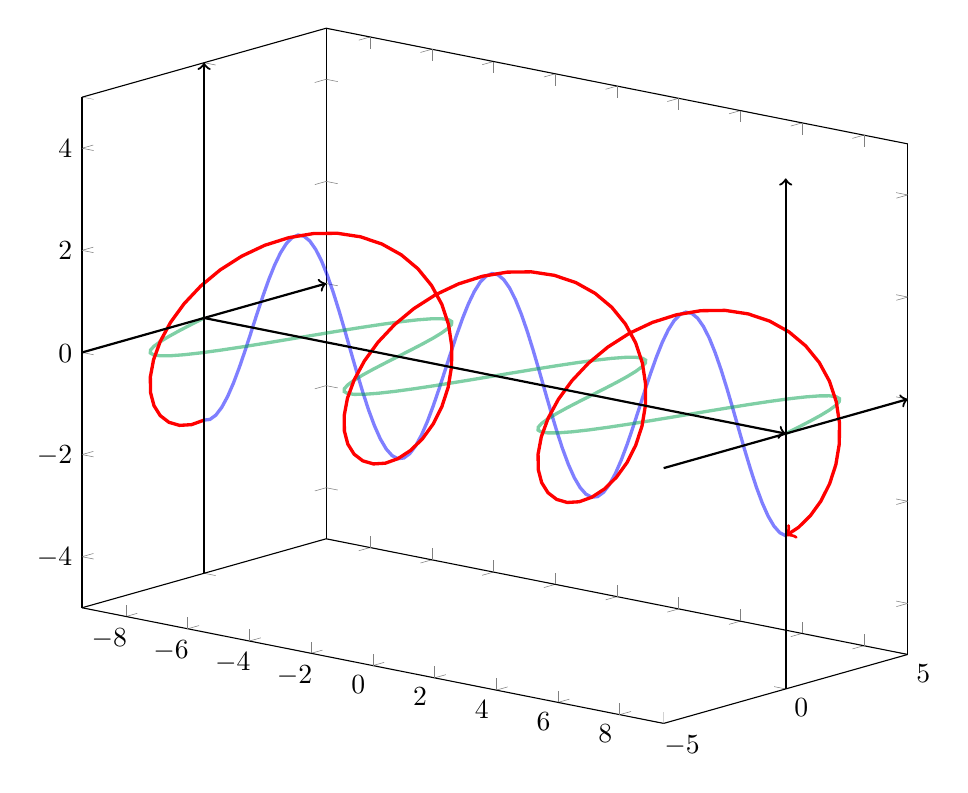
\begin{tikzpicture}
\begin{axis}[xmax=3*pi,ymax=5,xmin=-3*pi,ymin=-5,zmax=5,zmin=-5,view={40}{10},plot box ratio=2 1 1,
]


\addplot3+[blue,no markers,samples=100, samples y=0,domain=-3*pi:3*pi,variable=\t,style={very thick},opacity=0.5] ({\t},{0},{2*cos(\t r)});
\addplot3+[color1,no markers,samples=100, samples y=0,domain=-3*pi:3*pi,variable=\t,style={very thick},opacity=0.5] ({\t},{4*sin(\t r)},{0});
\addplot3+[red,no markers,samples=100, samples y=0,domain=-3*pi:3*pi,variable=\t,style={very thick},opacity=1,->] ({\t},{4*sin(\t r)},{2*cos(\t r)});

\addplot3+[black,no markers,samples=5, samples y=0,domain=-3*pi:3*pi,variable=\t,style={ thick,solid},->] ({\t},{0},{0});


\addplot3+[black,no markers,samples=100, samples y=0,domain=-5:5,variable=\t,style={ thick,solid},->] ({-3*pi},{\t},{0});
\addplot3+[black,no markers,samples=100, samples y=0,domain=-5:5,variable=\t,style={ thick,solid},->] ({3*pi},{\t},{0});

\addplot3+[black,no markers,samples=100, samples y=0,domain=-5:5,variable=\t,style={ thick,solid},->] ({-3*pi},{0},{\t});
\addplot3+[black,no markers,samples=100, samples y=0,domain=-5:5,variable=\t,style={ thick,solid},->] ({3*pi},{0},{\t});


%\addplot3+[black,no markers,samples=100, samples y=0,domain=-5:5,variable=\t,style={ thick}] ({3*pi},{-5},{\t});
%\addplot3+[black,no markers,samples=100, samples y=0,domain=-5:5,variable=\t,style={ thick}] ({3*pi},{\t},{5});
%\addplot3+[black,no markers,samples=5, samples y=0,domain=-3*pi:3*pi,variable=\t,style={ thick}] ({\t},{-5},{5});
\end{axis}

\end{tikzpicture}
\caption{luz elípticamente propagándose en el eje z}
\label{Fig:9.2.3.03}
\end{figure}

\subsection{Luz natural y parcialmente polarizada}

Los estados anteriores son estados puros que solo se dan para ondas ideales monocromáticas. En el caso de las ondas no monocromáticas las oscilaciones de las ondas electromagnéticas son mucho mas complejas, tal que los desfases dependen del tiempo $\varphi_x(t), \varphi_y (t)$. Sin pérdida generalidad podemos asumir que $\Delta \varphi = \varphi_y - \varphi_x$ tiene valores entre $0,2\pi$, lo cual es bastante lógico. \\

Si cada una de las fases individuales dependen del tiempo, la diferencia de fase ($\Delta \varphi$) también dependerá del tiempo. Sin embargo podemos considerar que es una función que varía lentamente con el tiempo en comparación con el argumento de la función $\omega t$. En ese caso en el entorno de un instante $t_0$ podemos considerar que $\delta(t_0)$ define el valor de $\delta$ en dicho entorno. En ese caso vamos a considerar lo siguiente cuando hablemos de \textbf{luz natural}:

\begin{itemize}
\item El desfase $\delta$ es una constante. Es decir, tendremos una polarización bien definida: circular, lineal o elíptica.
\item La variación de $\delta$ corresponde a una función equiprobable entre $0$ y $2 \pi$. No existe una componente privilegiada si ambas amplitudes son iguales.
\end{itemize}
En cualquier otro caso hablaremos de luz \textit{parcialmente polarizada}

\subsection{Álgebra de los estados de polarización lineal}

El álgebra de la polarización lineal es una forma muy divertida e interesante de expresar y estudiar como funciona la polarización de la luz. Lo que nos introducirá ahora nos permitirá resolver eficientemente como se comportan los polarizadores y la superposición de ondas con diferentes polarizaciones. \\

Como ya hemos dicho todo campo eléctrico debe vivir en el plano $XY$, y por tanto los  los vectores $\hnx$ y $\hny$ son una base del espacio de $\En$, ya que todo campo $\En$ posible lo podemos expresar como la suma de $\hnx$ y $\hny$. Esto se puede representar de forma matricial, tal que:

\begin{equation}
\hnx \equiv \begin{pmatrix}
1 \\
0
\end{pmatrix} \tquad
\hny \equiv \begin{pmatrix}
0 \\
1
\end{pmatrix}
\end{equation}

Dado que seguimos conservando las propiedades que deben conservarse, como puede ser $\hnx \cdot \hny = 0$, este cambio de notación es válido. Ahora expresamos un campo genérico usando este vector:

\begin{equation}
\En = e^{i(kz-\omega t)} \begin{pmatrix}
A_x \\
A_y e^{i \delta}
\end{pmatrix}
\end{equation}

De esta forma podemos expresar \textit{cualquier tipo de polarización}, siendo equivalente a lo visto anteriormente pero muchísimo mas fácil para trabajar. Ahora definimos el \textbf{vector de Jones} normalizado (puede que no este normalizado) tal que:

\begin{equation}
\Jn = \dfrac{1}{\sqrt{A_x^2 + A_y^2}} \begin{pmatrix}
A_x \\
A_y e^{i \delta}
\end{pmatrix}
\end{equation}

En la siguiente ecuación escribimos algunos ejemplos siendo: a) Luz linealmente polarizada en la dirección x=y. b) Luz circularmente polarizada levógira. c) Luz elípticamente polarizada:

\begin{equation}
a) \ \  \frac{1}{\sqrt{2}}
\begin{pmatrix}
1 \\
1 
\end{pmatrix} \tquad b) \ \  \frac{1}{\sqrt{2}} 
\begin{pmatrix}
1 \\
i
\end{pmatrix} \tquad c) \ \ \frac{1}{\sqrt{2}}  
\begin{pmatrix}
1 \\
e^{\frac{\pi}{4} i}
\end{pmatrix}
\end{equation}

\subsection{Álgebra de los polarizadores}

\subsubsection{Polarizadores}

Como ya hemos dicho expresar de manera matricial la polarización nos permite dar rienda suelta a todo nuestro conocimiento de álgebra lineal, como pueden ser los cambios de base o la diagonalización. \\

Llamamos a la dirección remanente tras el polarizador lineal el \textbf{eje del polarizador}, que nombramos como  $\un_\parallel$ o $\un$. Los campos así descritos pueden escribirse en cualquier otra base del espacio siempre que ambos vectores sean ortogonales (en realidad esto no haría ni falta, pero se supone ya que lo contrarío complicaría las cosas), tal que tenemos $\un$ y $\un_\perp$. Es decir:

\begin{equation}
\En = E_u \un  + E_\perp \un_\perp
\end{equation}
siendo $\theta$ el ángulo que forman $\En$ y $\un$ tendremos que:

\begin{equation}
\En = E \cos (\theta) \un + E \sin (\theta ) \un_\perp
\end{equation}

Todo esto parece obvio, y no os confundáis, \textit{lo es}, pero eso no evita que tengamos que mencionarlo. Es entonces claro que si polarizamos la luz en la dirección $\un$ de tal modo que al pasar tras dicho objeto óptico solo sobrevive la componente $\un$ del campo $\En$ original. Queda claro entonces que:

\begin{equation}
\En_{pol} = E \cos (\theta) \un
\end{equation}
tal que la irradiancia tras la acción del polarizador es:

\begin{equation}
I = \dfrac{1}{2} \varepsilon_0 c |\En \cdot \un |^2 = I_0 \cos^2 \theta
\end{equation}

\subsubsection{Matriz de Jones}

Ahora que sabemos como funciona un polarizador podremos usar matrices para estudiar la acción del polarización. Supongamos que un polarizador que deja pasar solo un vector $\un$ expresado de la siguiente forma matricialmente:

\begin{equation}
\un = \begin{pmatrix}
\cos \theta \\
\sin \theta 
\end{pmatrix}
\end{equation}
En ese caso nuestro polarizador tendrá deberá ser algún tipo de matriz que deje invariante dicho vector. El único que cumple estas condiciones es una matriz $2 \times 2$ que verifique que:

\begin{equation}
\begin{pmatrix}
\cos \theta \\
\sin \theta
\end{pmatrix} = \begin{pmatrix}
a & b \\ 
c & d 
\end{pmatrix}
\begin{pmatrix}
\cos \theta \\
\sin \theta
\end{pmatrix}
\end{equation}
Además debe anular cualquier vector perpendicular a $\un$, tal que:

\begin{equation}
\begin{pmatrix}
0 \\
0 
\end{pmatrix} = \begin{pmatrix}
a & b \\ 
c & d 
\end{pmatrix}
\begin{pmatrix}
\sin \theta \\
- \cos \theta
\end{pmatrix}
\end{equation}
Haciendo números llegamos a la expresión de la \textbf{matriz de Jones} que nos da la forma matricial para cualquier polarizador que solo permita pasar un vector $\un = \cos \theta \hnx + \sin \theta \hny$:

\begin{equation}
P(\theta) = \begin{pmatrix}
\cos^2 \theta & \cos \theta \sin \theta \\
\cos \theta \sin \theta & \sin^2 \theta
\end{pmatrix}
\end{equation}




\newpage

\section{Ondas electromagnéticas en medios anisótropos}

\subsection{Modelo microscópico del índice de refracción}

En un medio isótropo la disposición de los átomos no depende de la dirección, es exactamente igual en toda direccón. En los medios anisótropos esto no será asi, existe una diposición antisimétrica, de tal modo que las fuerzas de enlace que mantienen unidos los electrones varían según la dirección del movimiento de estos, y muchas veces ni siquiera están dirigidas en la dirección del movimiento. Una forma de ver esto es considerar las fuerzas de enlace diferentes para cada eje del sistema cartesiano. \\

Es otras palabras: existen diferentes $\Gamma$ y $\omega_0$ para cada dirección. Es esta anisitropía en las fuerzas de enlace y el comportamiento de los átomos del medio la que luego se manifiesta como una anisotropía del índice de refracciones. 


\subsection{Teoría electromagnética en los medios anisótropos}

\subsubsection{Características de las ondas electromagnéticas}

En el caso de las ondas planas tanto el gradiente como la derivada temporal se pueden expresar como \textit{operadores lineales complejos} tal que:

\begin{equation}
\nabla \rightarrow  i \kn \tquad \parciales{}{t} \rightarrow - i \omega
\end{equation}
de esta forma las ecuaciones de Maxwell quedan definidas de la siguiente forma:

\begin{subequations}
\begin{equation}
\nabla \Bn = 0 \longrightarrow i \kn \cdot \Bn = 0 \label{Ec:10.2.0.2a}
\end{equation}
\begin{equation}
\nabla \Dn = 0 \longrightarrow i \kn \cdot \Dn = 0
\end{equation}
\begin{equation}
\rota \Hn = \parciales{D}{t} \longrightarrow i \kn \ \times \Hn = - i \omega \Dn
\end{equation}
\begin{equation}
\rota \En = -\parciales{B}{t} \longrightarrow i \kn \ \times \En = i \omega \Bn
\end{equation}
\end{subequations}

El medio en este tema será no magnético $\Bn = \mu_0 \Hn$ (paralelos). De estas ecuaciones podemos extraer una información muy útil. En primer lugar tanto $\En$ como $\Dn$ viven en un plano perpendicular a $\Hn/\Bn$. Además  se verifica que $\Dn$ y $\kn$ son perpendiculares, y que $\Bn$ y $\kn$ también. Es decir, tenemos que $\Dn$ y $\Bn$ viven en un plano perpendicular a la \textit{dirección número de onda}. \\

Como podemos ver $\En$ y $\Dn$ paralelos no es una condición de las ecuaciones de Maxwell, y por tanto no tiene por qué verificarse para todos los medios. Entonces si $\Sn = \En \times \Hn$ y $\Dn \nparallel \En$, tendremos que $\Sn \nparallel \kn$. Es decir, existen una \textit{dirección del vector de ondas} ($\kn$) y una \textit{dirección de propagación de la onda} ($\Sn$) diferentes. 


\subsubsection{Tensor dieléctrico}

Hasta ahora hemos estudiado los medios lineales, isótropos y homogéneos. Estos medios verifican 3 propiedades: la relación entre $\Dn$ y $\En$ es puramente lineal ($\En \varpropto \Dn$), homogénea (se comporta igual en todo punto del medio) e isótropo (se comporta igual en toda dirección). Esto todo se puede escribir como $\En = \varepsilon \Dn$ donde $\varepsilon $ es una constante del medio. \\

Ahora vamos a estudiar otro tipo de medios los cuales mantienen la relación lineal y homogénea, perno no la isótropa. Es decir, en función de la dirección del campo, la relación entre $\Dn$ y $\En$ cambiará. Dado que el espacio solo tiene 3 direcciones independientes solo van a exisitir 3 constantes asociadas a cada uno de los elementos de la base del espacio (eje $x,y,z$) tal que:

\begin{equation}
D_x = \varepsilon_x E_x \quad D_y = \varepsilon_y E_y \quad D_z = \varepsilon_z E_z 
\end{equation}

Esto se podrá escribir de manera matricial, tal que si los campos se expresan como

\begin{equation}
\Dn \equiv \begin{pmatrix}
D_x \\
D_y  \\
D_z 
\end{pmatrix} \tquad \En \equiv \begin{pmatrix}
E_x \\
E_y \\
E_z
\end{pmatrix} 
\end{equation}
podemos crear un $\varepsilon$ matricial tal que:
\begin{equation}
\varepsilon = \begin{pmatrix}
\varepsilon_x & 0 & 0 \\
0 & \varepsilon_y & 0 \\
0 & 0 & \varepsilon_z 
\end{pmatrix}
\end{equation}
recuperando así la expresión 


\begin{equation}
\Dn = \varepsilon \En
\end{equation}
pero ahora con un significado mas profundo, general y potente. A esta matriz se la conoce como \textbf{tensor dieléctrico} y por tanto los campos dejan de ser vectores y pasan a ser \textit{tensores}. Podemos relacionar el tensor dieléctrico con un \textit{tensor índice de refracción} tal que si $n_k^2 = \varepsilon_k / \varepsilon_0$ tendremos que:


\begin{equation}
\varepsilon = \varepsilon_0 n^2 = \varepsilon_0 
\varepsilon = \begin{pmatrix}
n_x^2 & 0 & 0 \\
0 & n^2_y & 0 \\
0 & 0 & n^2_z 
\end{pmatrix}
\end{equation}
recuperando así la expresión $\varepsilon=\varepsilon_0 n^2$, que también hemos usado antes.



\subsubsection{Ecuación de Fresnel}

Las ecuación de ondas para ondas planas puede expresarse, si $\kn = n \frac{\omega}{c} \sn = n k_0 \sn$ (siendo $\sn$ el vector unitario, $n$ una constante tal que $v_p = c /n$, y $k_0 = \omega /c$), de la siguiente manera:

\begin{equation}
\kn \times ( \kn \times \En ) = - \omega^2  \dfrac{\varepsilon}{\varepsilon_0 c^2} \En
\end{equation}
Si usamos la relación $\an \times (\bn \times \cn) = (\an \cdot \cn) \bn - (\an \cdot \bn) \cn$ tendremos que:

\begin{equation}
\varepsilon_0 n^2 [(\sn \cdot \En) \sn - \En] + \varepsilon \En = 0 
\end{equation}
y por tanto tendremos que podemos separar por componentes la ecuación (recordemos que para medios anisótropos no se verifica que $\En \nvdash \kn$):

\begin{equation}
n^2 [ (\sn \cdot \En) s_k - E_k ] + n_k^2 E_k = 0 \label{Ec:10.2.3.10}
\end{equation}

Además aún queda una condición que se debe verificar: la relación $\Dn \cdot \sn  = \varepsilon_0 \sum n_k^2 E_k s_k = 0$. Si aplicamos esto en la ecuación anterior \ref{Ec:10.2.3.10} tendremos que:

\begin{equation}
\sum_k \dfrac{s_k^2}{\frac{1}{n^2}-\frac{1}{n_k^2}} \Longleftrightarrow \sum \dfrac{s_k^2}{v^2 - v_k^2} = 0
\end{equation}
donde $v=c/n,v_k = c/n_k$. Es entonces obvio que si nos dan una dirección de propagación $\sn$ podremos calcular los posibles índices de refracción, ya que desarrollando la ecuación (ignoramos el determinante):

\begin{equation}
s_x (v^2 - v_y^2)(v^2-v_z^2)+s_y (v^2 - v_x^2)(v^2-v_z^2)+s_z (v^2 - v_x^2)(v^2-v_y^2)=0 \label{Ec:10.2.3.12}
\end{equation}

Si por ejemplo tuviéramos que $\sn=(1,0,0)$ existen dos soluciones para $n$ que son $n=n_y$ o $n=n_z$. Para que se verifiquen las leyes de maxwell el campo eléctrico debe vibrar en cualquiera de esas dos direcciones. Si $\En$ vibra en $y$ o $z$, y $\Bn$ también (\ref{Ec:10.2.0.2a}) tendremos que $\sn \parallel \Sn$ y por tanto tendremos una expresión isótropa. \\


Una vez obtenidos los valores de los índices de refracción con la ecuación \ref{Ec:10.2.3.12} podemos obtener las direcciones de vibración de los campos eléctricos asociados a cada uno de los posibles valores del índice de refracción según la ecuación \ref{Ec:10.2.3.10}.


\subsubsection{Cristales uniáxicos}

Llamamos cristal uniáxico a aquel cristal que tiene un tensor dieléctrico  con dos valores coincidentes. Usamos el subíndice $o$ cuando nos referimos a las componentes iguales y $e$ cuando nos referimos a las componentes diferentes:

\begin{equation}
\varepsilon = \begin{pmatrix}
\varepsilon_0 & 0 & 0 \\
0 & \varepsilon_0 & 0 \\
0 & 0 & \varepsilon_e
\end{pmatrix} = \varepsilon_0 
\begin{pmatrix}
n^2_0 & 0 & 0 \\
0 & n^2_0 & 0 \\
0 & 0 & n^2_e 
\end{pmatrix}
\end{equation}

La dirección asociada a la constante dieléctrica diferente (extraordinaria) se le conoce por \textit{eje óptico}. Se distingue también los \textit{cristales uniáxicos positivos} con $n_e>n_o$ y los \textit{cristales uniáxicos negativos} con $n_e<n_o$. Supongamos por un segundo que el vector dirección de ondas forma un ángulo $\varphi$ con el eje óptico, de tal modo que la componente en el eje óptico (extraordinario) es $\cos \varphi$ y la componente en el eje ordinario por $\sin \theta$. En ese caso tendremos que:

\begin{equation}
\cos^2 \varphi (v^2 - v_o^2)(v^2-v_o^2)+ \sin^2 \varphi (v^2 - v_e^2)(v^2-v_o^2) = 0
\end{equation}
Como podemos ver una de las soluciones es que $n=n_o$, y otra de ellas es que:

$$ \cos^2 \varphi (v^2 - v_o^2)+ \sin ^2\varphi (v^2 - v_e^2) = 0 $$
Es entonces obvio que las posibles soluciones para el índice de refracción son:

\begin{equation}
n_1 = n_o \tquad \dfrac{1}{n_2^2} = \dfrac{\cos^2 \varphi}{n_0^2} + \dfrac{\sin^2 \varphi}{n_e^2} \label{Ec:10.2.4.15}
\end{equation}

Definimos como \textbf{plano principal} el plano que contiene el \textit{eje óptico} y a la dirección del vector de ondas $\sn$. La onda ordinaria es transversal: su campo eléctrico vibra perpendicularmente al plano principal. La onda extraordinaria no es (en general) trasversal: su campo eléctrico vibra contenido en el plano principal.

\subsubsection{Birreflejancia}


La refracción en la frontera de un cristal anisótropo tiene unas características peculiares, que dependen de los valores del índice de refracción principales como de la orientación de la superficie de frontera con respecto a la estructura del cristal, con las siguientes características:

\begin{itemize}
\item La onda incidente genera dos ondas en diferentes direcciones, siendo estas ondas linealmente polarizadas ortogonales (sea cual sea el estado de polarización inicial).

\item Una de las dos ondas no puede estar contenida en el plano de incidencia.
\item La desviación de la luz puede ocurrir incluso en el caso de la incidencia normal.
\end{itemize}

En general la ley de Snell se verificará de manera separada para cada onda. Si suponemos que la onda incide desde el aire $n_1=1$. Si escribimos $n$ como el índice de refracción del medio tendremos que:

\begin{equation}
\sin \theta_1 = n \sin \theta_2 \label{Ec:10.2.5.14}
\end{equation}
siendo $n=n_o$ para la \textit{onda ordinaria} y siendo $n=n(\varphi)$ para la \textit{onda extraordinaria}. Podemos reescribir $\varphi$ en función del ángulo $\theta_2$ y el ángulo $\alpha$ que nos da \textit{el ángulo que forma el eje óptico y la normal de la superficie frontera}. En ese caso:

\begin{equation}
\varphi = \theta_2 + \alpha
\end{equation}

La resolución de la ecuación \ref{Ec:10.2.5.14} nos permite obtener los índices de refracción de las ondas y la dirección de $\kn$. A partir de esto podremos obtener el valor de ambos campos y las direcciones de propagación de la energía a partir del valor de la onda incidente. \\

Un caso muy curioso es el caso de la incidencia normal. Mientras que la onda ordinaria no se desvía; pero el caso de la onda extraordinaria si se desviará ya que la dirección es dada por $\varphi$. 


\subsection{Dispositivos birreflejantes}

Los polarizadores birreflejantes están formados por dos prismas rectangulares, de tal manera que las ondas que se propagan en el primer prisma se reflactan de diferente forma en el segundo prisma.

\subsubsection{Laminas de retardo}

Las láminas de retardo son dispositivos que transforman el estado de polarización de un haz ya polarizado. Se construyen por dos láminas finas de cristal anisótropo con dos ejes principales contenidos en la superficie frontal. En el caso de un cristal uniáxico es suficiente con que el eje óptico este contenido en esa superficie. Dado que la onda incidente no se desvía, en la lámina se originan dos ondas que se propagan con diferente velocidad de fase por lo que se creará una diferencia de fase entre ellas. Si consideramos un cristal biáxico de espesor $d$, denotando $n_x$ y $n_y$ los índices principales asociados con los ejes contenidos en la superficie de la lámina, se expresa el desfase como:

\begin{equation}
\Delta \varphi = \frac{2 \pi}{\lambda} (n_y - n_x) d
\end{equation}
o en el caso de un cristal uniáxico:

\begin{equation}
\Delta \varphi = \dfrac{2 \pi}{\lambda} (n_e - n_o ) d 
\end{equation}

Si el eje óptico no se encuentra en uno de los ejes que forman parte de la superficie de separación entonces no tendríamso $n_e$ si no $n_2$ calculado con la ecuación \ref{Ec:10.2.4.15}. \\

Dado que la salida del cristal produce un cambio tal que solo modifica la fase entre ondas y no su dirección, podremos usar la siguiente \textit{matriz de Jones} para describir este tipo de polarizadores:

\begin{equation}
J = e^{\varphi_x} 
\begin{pmatrix}
1 & 0 \\
0 & e^{i \Delta \varphi}
\end{pmatrix}
\end{equation}

Existen dos láminas de retardo ampliamente usadas, que sirven para convertir un haz linealmente polarizado en un haz circular/elípticamente polarizado. Estas son:

\begin{itemize}
\item  \textbf{Lámina de cuarto de onda:} esta lámina lo que hace es dar un retraso de $\pi/2$ a uno de los ejes. De este modo debe verificarse que $\Delta \varphi = (2n+1) \pi / 2$ con $n\in \mathbb{Z}$, de tal modo que:

\begin{equation}
\lambda_n = \dfrac{4}{2n+1} d \Delta n 
\end{equation}
Esta lámina puede convertir una onda linealmente polarizada en un haz elíptico/circular al desfasar $\pi/2$ uno de los ejes. Si la onda saliente es circularmente polarizada o elípticamente polarizada lo decidirán los ángulos entre la luz incidente y los ejes que se retrasan y las amplitudes de estos. También es capaz de convertir una onda circular en una onda linealmente polarizada.

\item \textbf{Lámina de media onda:} en este caso el desfase introducido es de $\pi$, de tal modo que si $\Delta \varphi  = (2n+1) \pi$, tendremos que:


\begin{equation}
\lambda_n = \dfrac{2}{2n+1} d \Delta n 
\end{equation}
Esta lámina invierte uno de los ejes de vibración del campo eléctrico, por lo que es capaz de convertir una onda linealmente polarizada incidente en una onda linealmente polarizada perpendicular a esta; o una onda circular levógira en una dextrógira. 
\end{itemize}

\subsubsection{Compensador de Babinet}

El \textbf{compensador de Babinet} es un objeto formado por los cristales uniáxicos con con ejes intercambiados (si en uno $n_e$ va en el $\hnx$, en el otro $n_e$ irá en el $\hny$). En ese caso tendremos que las fases se \textit{compensan}, de tal modo que:


\begin{equation}
\Delta \varphi = \dfrac{2 \pi}{\lambda} (n_e - n_o ) (d_2-d_1)
\end{equation}
Ahora bien ¿Cuál es la ultilidad de esto? Pues que si $d_2$ y $d_1$ varían en función de la posición en la que incida el rayo normal tendremos una lamina retardadora variable y fácilmente ajustable. Para que sea así el objeto debe estar construido como en la imagen \ref{Fig:10.3.1.01} con un ángulo $\alpha$ sumamente pequeño para que prácticamente no haya desviación (típicamente $\alpha < 2,5º$). 

\begin{figure}[h!] \centering
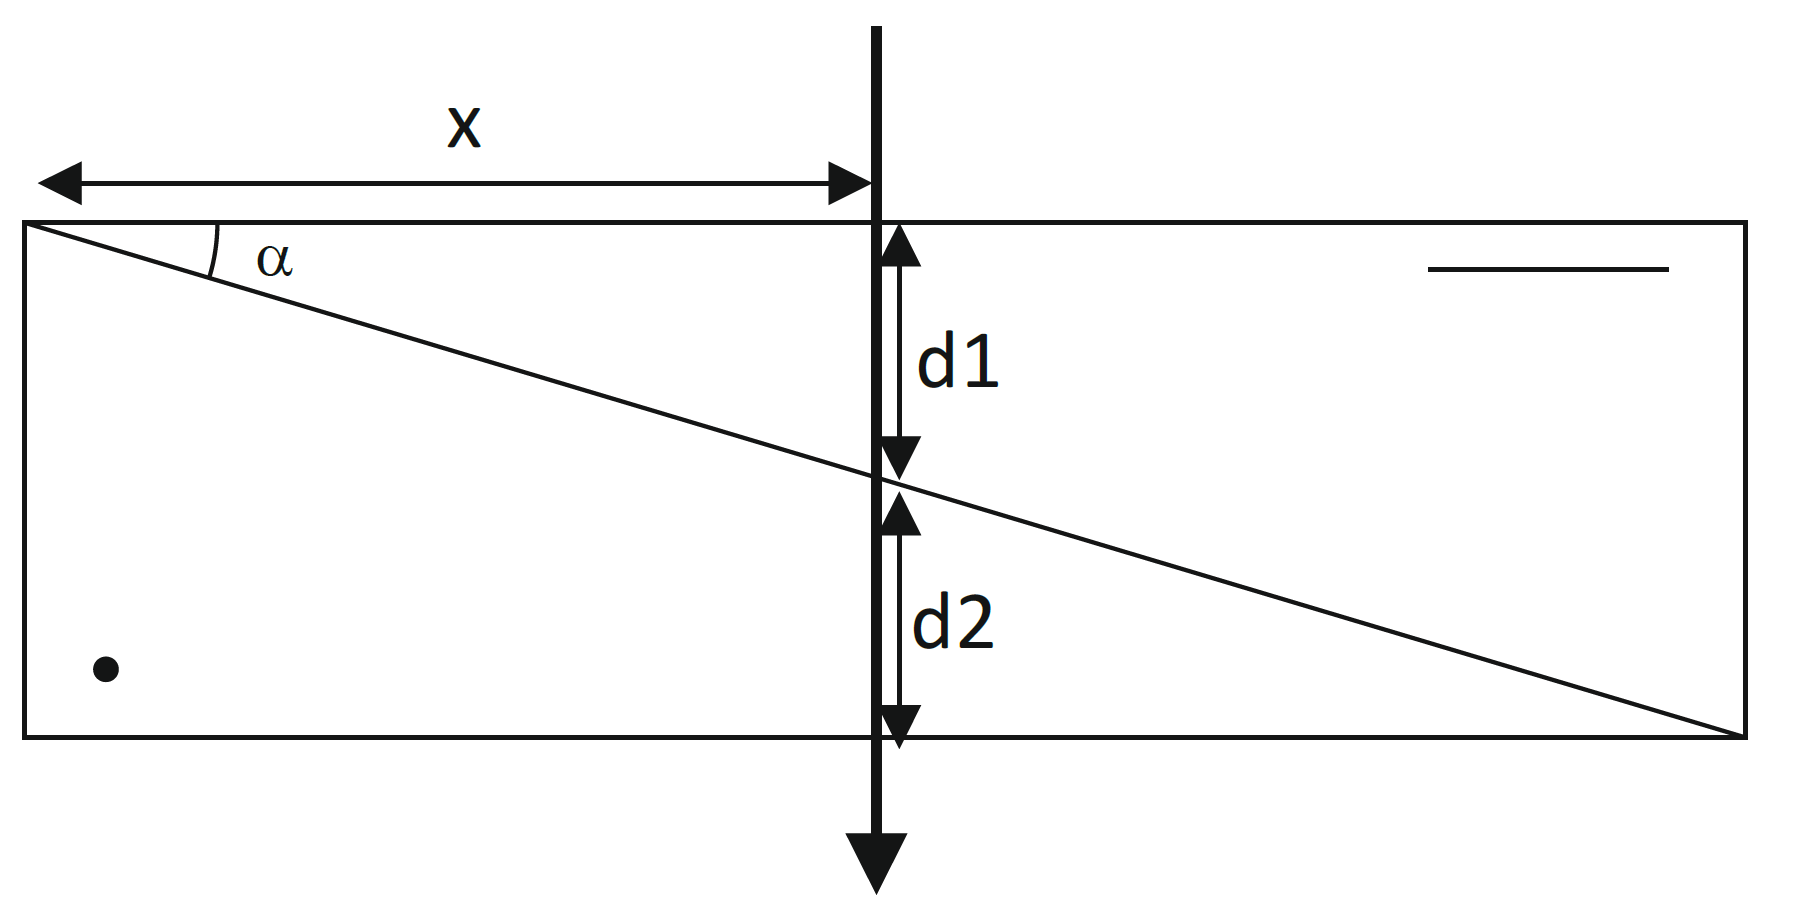
\includegraphics[scale=0.4]{Babinet.png}
\caption{Compensador de Babinet.}
\label{Fig:10.3.1.01}
\end{figure}


\end{document}